\documentclass[a4paper, 12pt]{report}		% general format
\usepackage{multicol}
%%%% Charset
\usepackage{cmap}							% make PDF files searchable and copyable
\usepackage{bm}
\usepackage{pdfpages}
\usepackage[utf8x]{inputenc} 				% accept different input encodings
\usepackage[english,russian]{babel}   %% загружает пакет многоязыковой вёрстки
%\usepackage{fontspec}      %% подготавливает загрузку шрифтов Open Type, True Type и др.
%\defaultfontfeatures{Ligatures={TeX},Renderer=Basic}  %% свойства шрифтов по умолчанию
%\setmainfont[Ligatures={TeX,Historic}]{Roboto-Light} %% задаёт основной шрифт документа
%\setsansfont{Roboto-Light}  
\usepackage{float}
%%%% Graphics
%\usepackage[dvipsnames]{xcolor}			% driver-independent color extensions
\usepackage{graphicx}						% enhanced support for graphics
\usepackage{wrapfig}						% produces figures which text can flow around

%%%% Math
\usepackage{amsmath}						% American Mathematical Society (AMS) math facilities
\usepackage{amsfonts}						% fonts from the AMS
\usepackage{amssymb}						% additional math symbols

%%%% Typograpy (don't forget about cm-super)
\usepackage{microtype}						% subliminal refinements towards typographical perfection
\linespread{1.0}							% line spacing
\usepackage[mag=1000, left=2.0cm, right=1.5cm, top=2cm, bottom=2cm, headsep=0.7cm, footskip=1cm]{geometry}
\setlength{\parindent}{0pt}					% we don't want any paragraph indentation
\usepackage{parskip}						% some distance between paragraphs

%%%% Tables
\usepackage{tabularx}						% tables with variable width columns
\usepackage{multirow}						% for tabularx
\usepackage{hhline}							% for tabularx
\usepackage{tabu}
\usepackage{longtable}

%%%% Graph
\usepackage{tikz}							% package for creating graphics programmatically
\usetikzlibrary{arrows}						% edges for tikz

%%%% Other
\usepackage{url}							% verbatim with URL-sensitive line breaks
\usepackage{fancyvrb}						% sophisticated verbatim text (with box)

\usepackage{fancyhdr}
\usepackage{latexsym}
\usepackage{booktabs}
\usepackage{array}

\usepackage{listings}
\usepackage{caption}
\DeclareCaptionFont{white}{\color{white}}
\DeclareCaptionFormat{listing}{\colorbox{gray}{\parbox{\dimexpr\textwidth-1.72\fboxsep\relax}{#1#2#3}}}
\captionsetup[lstlisting]{format=listing,labelfont=white,textfont=white,margin=0pt}
\lstset{language=C,
	basicstyle=\footnotesize,
	keepspaces=true,
	tabsize=4,               
	frame=single,                           % Single frame around code
	rulecolor=\color{black},
	captionpos=b,
	showstringspaces=false,	
	abovecaptionskip=-0.9pt,
	xleftmargin=3.4pt,
	xrightmargin=2.6pt,
	breaklines=true,
	postbreak=\raisebox{0ex}[0ex][0ex]{\ensuremath{\color{black}\hookrightarrow\space}},
	xleftmargin=3.2pt,
	literate={а}{{\selectfont\char224}}1
	{~}{{\textasciitilde}}1
	{б}{{\selectfont\char225}}1
	{в}{{\selectfont\char226}}1
	{г}{{\selectfont\char227}}1
	{д}{{\selectfont\char228}}1
	{е}{{\selectfont\char229}}1
	{ё}{{\"e}}1
	{ж}{{\selectfont\char230}}1
	{з}{{\selectfont\char231}}1
	{и}{{\selectfont\char232}}1
	{й}{{\selectfont\char233}}1
	{к}{{\selectfont\char234}}1
	{л}{{\selectfont\char235}}1
	{м}{{\selectfont\char236}}1
	{н}{{\selectfont\char237}}1
	{о}{{\selectfont\char238}}1
	{п}{{\selectfont\char239}}1
	{р}{{\selectfont\char240}}1
	{с}{{\selectfont\char241}}1
	{т}{{\selectfont\char242}}1
	{у}{{\selectfont\char243}}1
	{ф}{{\selectfont\char244}}1
	{х}{{\selectfont\char245}}1
	{ц}{{\selectfont\char246}}1
	{ч}{{\selectfont\char247}}1
	{ш}{{\selectfont\char248}}1
	{щ}{{\selectfont\char249}}1
	{ъ}{{\selectfont\char250}}1
	{ы}{{\selectfont\char251}}1
	{ь}{{\selectfont\char252}}1
	{э}{{\selectfont\char253}}1
	{ю}{{\selectfont\char254}}1
	{я}{{\selectfont\char255}}1
	{А}{{\selectfont\char192}}1
	{Б}{{\selectfont\char193}}1
	{В}{{\selectfont\char194}}1
	{Г}{{\selectfont\char195}}1
	{Д}{{\selectfont\char196}}1
	{Е}{{\selectfont\char197}}1
	{Ё}{{\"E}}1
	{Ж}{{\selectfont\char198}}1
	{З}{{\selectfont\char199}}1
	{И}{{\selectfont\char200}}1
	{Й}{{\selectfont\char201}}1
	{К}{{\selectfont\char202}}1
	{Л}{{\selectfont\char203}}1
	{М}{{\selectfont\char204}}1
	{Н}{{\selectfont\char205}}1
	{О}{{\selectfont\char206}}1
	{П}{{\selectfont\char207}}1
	{Р}{{\selectfont\char208}}1
	{С}{{\selectfont\char209}}1
	{Т}{{\selectfont\char210}}1
	{У}{{\selectfont\char211}}1
	{Ф}{{\selectfont\char212}}1
	{Х}{{\selectfont\char213}}1
	{Ц}{{\selectfont\char214}}1
	{Ч}{{\selectfont\char215}}1
	{Ш}{{\selectfont\char216}}1
	{Щ}{{\selectfont\char217}}1
	{Ъ}{{\selectfont\char218}}1
	{Ы}{{\selectfont\char219}}1
	{Ь}{{\selectfont\char220}}1
	{Э}{{\selectfont\char221}}1
	{Ю}{{\selectfont\char222}}1
	{Я}{{\selectfont\char223}}1,
	extendedchars=true
}

%галочка
\usepackage{amssymb}% http://ctan.org/pkg/amssymb
\usepackage{pifont}% http://ctan.org/pkg/pifont
\newcommand{\cmark}{\ding{52}}%
\newcommand{\xmark}{\ding{56}}
%------------------------------------------------------------------------------
\renewcommand{\labelenumii}{\theenumii}
\renewcommand{\theenumii}{\theenumi.\arabic{enumii}.}
\addto\captionsrussian{\def\refname{Список использованных источников}}
\begin{document}
\begin{titlepage}
\thispagestyle{empty}

\begin{center}
Санкт-Петербургский политехнический университет Петра Великого\\
Институт Информационных Технологий и Управления\\*
Кафедра компьютерных систем и программных технологий\\*
\hrulefill
\end{center}

\vspace{15em}

\begin{center}
\textsc{\textbf{Курсовая работа}}
\vspace{1em}

Дисциплина: \textbf{Методы оптимизации}
\vspace{2em}

Тема: \textbf{Формулировка и решение задачи выбора оптимального решения с использованием различных математических моделей}
\end{center}

\vspace{16em}

\begin{flushleft}
Выполнил студент гр. 53501/3 \hrulefill С.А. Мартынов \\
\vspace{1.5em}
Руководитель, к.т.н.,доц. \hrulefill А.Г. Сиднев\\
\end{flushleft}

\vspace{\fill}

\begin{center}
Санкт-Петербург \\
2015
\end{center}

\end{titlepage}
\setcounter{page}{2}
%
\includepdf[pages=-,pagecommand={},width=\textwidth]{task.pdf}
\tableofcontents
\clearpage

%------------------------------------------------------------------------------
%\input{intro}

\addcontentsline{toc}{chapter}{Введение}
\chapter*{Введение}
В данной работе рассматриваются следующие задачи:
\begin{enumerate}
\item Формализация многокритериальной оптимизационной задачи, методы сведения к однокритериальной, решение с использованием Optimization Toolbox системы Matlab;
\item Поиск оптимальной стратегии принятия решений с использованием марковских моделей;
\item Оптимизация сетей систем массового обслуживания;
\item Решение задачи анализа потокового графа с использованием методики GERT и алгебры потоковых графов.
\end{enumerate}

\documentclass[a4paper, 12pt]{report}		% general format
\usepackage{multicol}
%%%% Charset
\usepackage{cmap}							% make PDF files searchable and copyable
\usepackage{bm}
\usepackage{pdfpages}
\usepackage[utf8x]{inputenc} 				% accept different input encodings
\usepackage[english,russian]{babel}   %% загружает пакет многоязыковой вёрстки
%\usepackage{fontspec}      %% подготавливает загрузку шрифтов Open Type, True Type и др.
%\defaultfontfeatures{Ligatures={TeX},Renderer=Basic}  %% свойства шрифтов по умолчанию
%\setmainfont[Ligatures={TeX,Historic}]{Roboto-Light} %% задаёт основной шрифт документа
%\setsansfont{Roboto-Light}  
\usepackage{float}
%%%% Graphics
%\usepackage[dvipsnames]{xcolor}			% driver-independent color extensions
\usepackage{graphicx}						% enhanced support for graphics
\usepackage{wrapfig}						% produces figures which text can flow around

%%%% Math
\usepackage{amsmath}						% American Mathematical Society (AMS) math facilities
\usepackage{amsfonts}						% fonts from the AMS
\usepackage{amssymb}						% additional math symbols

%%%% Typograpy (don't forget about cm-super)
\usepackage{microtype}						% subliminal refinements towards typographical perfection
\linespread{1.0}							% line spacing
\usepackage[mag=1000, left=2.0cm, right=1.5cm, top=2cm, bottom=2cm, headsep=0.7cm, footskip=1cm]{geometry}
\setlength{\parindent}{0pt}					% we don't want any paragraph indentation
\usepackage{parskip}						% some distance between paragraphs

%%%% Tables
\usepackage{tabularx}						% tables with variable width columns
\usepackage{multirow}						% for tabularx
\usepackage{hhline}							% for tabularx
\usepackage{tabu}
\usepackage{longtable}

%%%% Graph
\usepackage{tikz}							% package for creating graphics programmatically
\usetikzlibrary{arrows}						% edges for tikz

%%%% Other
\usepackage{url}							% verbatim with URL-sensitive line breaks
\usepackage{fancyvrb}						% sophisticated verbatim text (with box)

\usepackage{fancyhdr}
\usepackage{latexsym}
\usepackage{booktabs}
\usepackage{array}

\usepackage{listings}
\usepackage{caption}
\DeclareCaptionFont{white}{\color{white}}
\DeclareCaptionFormat{listing}{\colorbox{gray}{\parbox{\dimexpr\textwidth-1.72\fboxsep\relax}{#1#2#3}}}
\captionsetup[lstlisting]{format=listing,labelfont=white,textfont=white,margin=0pt}
\lstset{language=C,
	basicstyle=\footnotesize,
	keepspaces=true,
	tabsize=4,               
	frame=single,                           % Single frame around code
	rulecolor=\color{black},
	captionpos=b,
	showstringspaces=false,	
	abovecaptionskip=-0.9pt,
	xleftmargin=3.4pt,
	xrightmargin=2.6pt,
	breaklines=true,
	postbreak=\raisebox{0ex}[0ex][0ex]{\ensuremath{\color{black}\hookrightarrow\space}},
	xleftmargin=3.2pt,
	literate={а}{{\selectfont\char224}}1
	{~}{{\textasciitilde}}1
	{б}{{\selectfont\char225}}1
	{в}{{\selectfont\char226}}1
	{г}{{\selectfont\char227}}1
	{д}{{\selectfont\char228}}1
	{е}{{\selectfont\char229}}1
	{ё}{{\"e}}1
	{ж}{{\selectfont\char230}}1
	{з}{{\selectfont\char231}}1
	{и}{{\selectfont\char232}}1
	{й}{{\selectfont\char233}}1
	{к}{{\selectfont\char234}}1
	{л}{{\selectfont\char235}}1
	{м}{{\selectfont\char236}}1
	{н}{{\selectfont\char237}}1
	{о}{{\selectfont\char238}}1
	{п}{{\selectfont\char239}}1
	{р}{{\selectfont\char240}}1
	{с}{{\selectfont\char241}}1
	{т}{{\selectfont\char242}}1
	{у}{{\selectfont\char243}}1
	{ф}{{\selectfont\char244}}1
	{х}{{\selectfont\char245}}1
	{ц}{{\selectfont\char246}}1
	{ч}{{\selectfont\char247}}1
	{ш}{{\selectfont\char248}}1
	{щ}{{\selectfont\char249}}1
	{ъ}{{\selectfont\char250}}1
	{ы}{{\selectfont\char251}}1
	{ь}{{\selectfont\char252}}1
	{э}{{\selectfont\char253}}1
	{ю}{{\selectfont\char254}}1
	{я}{{\selectfont\char255}}1
	{А}{{\selectfont\char192}}1
	{Б}{{\selectfont\char193}}1
	{В}{{\selectfont\char194}}1
	{Г}{{\selectfont\char195}}1
	{Д}{{\selectfont\char196}}1
	{Е}{{\selectfont\char197}}1
	{Ё}{{\"E}}1
	{Ж}{{\selectfont\char198}}1
	{З}{{\selectfont\char199}}1
	{И}{{\selectfont\char200}}1
	{Й}{{\selectfont\char201}}1
	{К}{{\selectfont\char202}}1
	{Л}{{\selectfont\char203}}1
	{М}{{\selectfont\char204}}1
	{Н}{{\selectfont\char205}}1
	{О}{{\selectfont\char206}}1
	{П}{{\selectfont\char207}}1
	{Р}{{\selectfont\char208}}1
	{С}{{\selectfont\char209}}1
	{Т}{{\selectfont\char210}}1
	{У}{{\selectfont\char211}}1
	{Ф}{{\selectfont\char212}}1
	{Х}{{\selectfont\char213}}1
	{Ц}{{\selectfont\char214}}1
	{Ч}{{\selectfont\char215}}1
	{Ш}{{\selectfont\char216}}1
	{Щ}{{\selectfont\char217}}1
	{Ъ}{{\selectfont\char218}}1
	{Ы}{{\selectfont\char219}}1
	{Ь}{{\selectfont\char220}}1
	{Э}{{\selectfont\char221}}1
	{Ю}{{\selectfont\char222}}1
	{Я}{{\selectfont\char223}}1,
	extendedchars=true
}

%галочка
\usepackage{amssymb}% http://ctan.org/pkg/amssymb
\usepackage{pifont}% http://ctan.org/pkg/pifont
\newcommand{\cmark}{\ding{52}}%
\newcommand{\xmark}{\ding{56}}
%------------------------------------------------------------------------------
\renewcommand{\labelenumii}{\theenumii}
\renewcommand{\theenumii}{\theenumi.\arabic{enumii}.}
\addto\captionsrussian{\def\refname{Список использованных источников}}
\begin{document}
\begin{titlepage}
\thispagestyle{empty}

\begin{center}
Санкт-Петербургский политехнический университет Петра Великого\\
Институт Информационных Технологий и Управления\\*
Кафедра компьютерных систем и программных технологий\\*
\hrulefill
\end{center}

\vspace{15em}

\begin{center}
\textsc{\textbf{Курсовая работа}}
\vspace{1em}

Дисциплина: \textbf{Методы оптимизации}
\vspace{2em}

Тема: \textbf{Формулировка и решение задачи выбора оптимального решения с использованием различных математических моделей}
\end{center}

\vspace{16em}

\begin{flushleft}
Выполнил студент гр. 53501/3 \hrulefill С.А. Мартынов \\
\vspace{1.5em}
Руководитель, к.т.н.,доц. \hrulefill А.Г. Сиднев\\
\end{flushleft}

\vspace{\fill}

\begin{center}
Санкт-Петербург \\
2015
\end{center}

\end{titlepage}
\setcounter{page}{2}
\tableofcontents
\clearpage

%------------------------------------------------------------------------------
%\input{intro}
\chapter{МНОГОКРИТЕРИАЛЬНАЯ ОПТИМИЗАЦИЯ}
\section{Постановка задачи}
\subsection{Индивидуальное задание}
\textbf{Задача 2}\\
Фабрика производит два вида изделий, А и Б. Продажа изделий осуществляется на внутреннем рынке и также экспортируется в другие страны. Стоимость изделия А на внутреннем рынке \$30, а на внешнем - \$45, стоимость изделия Б на внутреннем рынке \$20, а на внешнем - \$21.

Для изготовления изделий используются два вида станков. Для изготовления 1 единицы изделия А необходима работа первого станка в течении 1 часа и второго – в течение 2 часов, а для изготовления 1 единицы изделия Б необходима работы первого станка в течение 5 часов и второго в течение 7 часов. Ресурс времени непрерывной работы 1 станка 18 часов, а 2 – 20 часов. 

Изучение рынка сбыта показало, что спрос на изделие А никогда не превышает 5000 изделий в сутки, а на изделие Б - 9000. 

Какое количество изделий каждого вида надо производить в  данных условиях для внутреннего и для внешнего рынков, чтобы доход от реализации продукции на внутреннем рынке был максимальным?  Какое количество изделий каждого вида надо производить, чтобы минимизировать время использования станков при  условии использования не менее 80\% ресурса непрерывной работы каждого станка? Какое количество изделий каждого вида надо производить в  данных условиях, чтобы доход от реализации продукции на экспорт был максимальным?

\subsection{Пункты расчетного задания}
\begin{enumerate}
\item Осуществить переход от многокритериальной задачи к однокритериальной с использованием следующих подходов:
\begin{itemize}
\item Выделение главного критерия;
\item Свертка критериев (аддитивная и мультипликативная);
\item Максимин или минимакс (он же метод максиминной свертки);
\item Метод последовательных уступок;
\item fgoalattain;
\item Ведение метрики в пространстве критериев.
\end{itemize}
\item Решить задачу стохастического программирования для одной из однокритериальных задач, превратив детерминированное ограничение в вероятностное по схеме
\end{enumerate}
\begin{equation}
P(\sum_{j=1}^{n} a_{ij}x_j-b_i\leq 0)\geq a_i
\end{equation}
Менять $a_i$ в следующем диапазоне $0,1\leq a_i\leq 0,9$
 
Считать случайной величиной $b_i$ или элементы ${a_{ij} i}$-й строки матрицы $A{a_{ij}}$ (по выбору).
%\pmb{$$}

\section{Математическая модель задачи многокритериальной оптимизации}
\begin{itemize}
\item $x_{11}$ – количество изделий А на внутреннем рынке;
\item $x_{12}$ – количество изделий A на внешнем рынке;
\item $x_{21}$ – количество изделий Б на внутреннем рынке;
\item $x_{22}$ – количество изделий Б на внешнем рынке.
\end{itemize}
\textbf{Первый критерий}. Максимизация дохода на внутреннем рынке
\begin{equation}
f_1 (x_{11}, x_{21})=30*x_{11}+20*x_{21} \rightarrow max 
\end{equation}
\textbf{Второй критерий}. Минимизация использования станков

\begin{equation}
\begin{split}
f_2 (x_{11}, x_{12}, x_{21}, x_{22})=\\ &
\left(x_{11}+x_{12})+2*(x_{11}+x_{12})+5*(x_{21}+x_{22})+7*(x_{21}+x_{22}\right)=\\ & 
3*\left(x_{11}+x_{12})+12*(x_{21}+x_{22}\right) \rightarrow min
\end{split}
\end{equation}
\textbf{Третий критерий}. Максимизация дохода на внешнем рынке
\begin{equation}
f_3 (x_{12}, x_{22})= 45*x_{12}+21*x_{22} \rightarrow max
\end{equation}
\textbf{Примечание: решений, с ограничением на использование не менее 80\% ресурса непрерывной работы станков, найти не удалось. Поэтому данное ограничение было снижено до 70\%.}\\
\textbf{Также часы были переведены в минуты.}\\\\
\textbf{Ограничения:}\\
Для станков первого типа
\begin{equation}
1*(x_{11}+x_{12})+5*(x_{21}+x_{22})\leq 18*60
\end{equation}
\begin{equation} \label{limit:1}
1*(x_{11}+x_{12})+5*(x_{21}+x_{22})\geq (18*60)*0.7
\end{equation}
Для станков второго типа
\begin{equation}
2*(x_{11}+x_{12})+7*(x_{21}+x_{22})\leq 20*60
\end{equation}
\begin{equation} \label{limit:2}
2*(x_{11}+x_{12})+7*(x_{21}+x_{22})\geq (20*60)*0.7
\end{equation}
Ограничения по количеству изделий
\begin{equation}
\begin{cases}
x_{11}+x_{12}\leq 5000\\
x_{21}+x_{22}\leq 9000
\end{cases}
\end{equation}
С учетом требований пакета MATLAB к постановке задач оптимизации, необходимо представить целевые функции как поиск минимумов, а ограничения записать в виде $g(x) \leq 0$. Изменим ограничения \ref{limit:1} и \ref{limit:2}, а также введем новые функции, где $z_1=-f_1, z_3=-f_3$. В итоге получим:
\begin{equation}
z_1 (x_{11}, x_{21})=-(30*x_{11}+20*x_{21}) \rightarrow min 
\end{equation}
\begin{equation}
z_3 (x_{12}, x_{22})= -(45*x_{12}+21*x_{22}) \rightarrow min
\end{equation}
\textbf{Ограничения:}
\begin{equation}
\begin{cases}
1*(x_{11}+x_{12})+5*(x_{21}+x_{22})\leq 18*60\\
-1*(x_{11}+x_{12})-5*(x_{21}+x_{22})\leq -(18*60)*0.7\\
2*(x_{11}+x_{12})+7*(x_{21}+x_{22})\leq 20*60\\
-2*(x_{11}+x_{12})-7*(x_{21}+x_{22})\leq -(20*60)*0.7\\
x_{11}+x_{12}\leq 5000\\
x_{21}+x_{22}\leq 9000
\end{cases}
\end{equation}
\subsection{Поиск оптимумов частных критериев}
Найдем оптимумы каждой из целевых функций независимо от других. Для этого необходимо решить три задачи однокритериальной оптимизации: для $z_1, f_2, z_3$ при тех же ограничениях на $x_{11}, x_{12}, x_{21}, x_{22}$ что имеют место для задачи многокритериальной оптимизации.

Для решение данной задачи, был использован MATLAB.
\begin{lstlisting}[language={matlab}, caption={Скрипт с общими параметрами}, label={lst:0}]
clc; clearvars
% Параметры
Tmin1 = (18*60)*0.7;  %Минимально допустимое время работы 1 станка
Tmin2 = (20*60)*0.7;  %Минимально допустимое время работы 2 станка
Tmax1 = (18*60);  %Максимально допустимое время работы 1 станка
Tmax2 = (20*60);  %Максимально допустимое время работы 2 станка

% Целевые функции
f1 = @(X) 30*X(1) + 20*X(3); % -> max
f2 = @(X) 3*(X(1)+X(2))+12*(X(3)+X(4)); % -> min
f3 = @(X) 45*X(2) + 21*X(4); % -> max

z1 = @(N) -f1(N); % -> min
z3 = @(N) -f3(N); % -> min

% Функциональные ограничения (в данном случае только линейные)
A = [1,1,5,5;
    -1,-1,-5,-5;
    2,2,7,7;
    -2,-2,-7,-7;
    1,1,0,0;
    0,0,1,1];
b = [Tmax1; -Tmin1; Tmax2; -Tmin2;  5000; 9000];

Aeq = [];
beq = [];
% Параметрические ограничения
lb = [0; 0; 0; 0];
ub = [5000; 5000; 9000; 9000];
\end{lstlisting}

\begin{lstlisting}[language={matlab}, caption={Поиск оптимумов частных критериев}, label={lst:1}]
%% Поиск оптимумов частных критериев
startingPoint = lb;
[x, z1_opt] = fmincon(z1, startingPoint, A, b, Aeq, beq, lb, ub)
[x, f2_opt] = fmincon(f2, startingPoint, A, b, Aeq, beq, lb, ub)
[x, z3_opt] = fmincon(z3, startingPoint, A, b, Aeq, beq, lb, ub)
\end{lstlisting}

\begin{lstlisting}[language={matlab}, caption={Результаты выполнения листинга \ref{lst:1}}]
x =
  236.0000
    0.0000
  104.0000
    0.0000
z1_opt =
  -9.1600e+03

x =
    0.0000
    0.0000
   75.6000
   75.6000
f2_opt =
   1.8144e+03

x =
  0.0000
  236.0000
  0.0000
  104.0000

z3_opt =
  -1.2804e+04

\end{lstlisting}
Таким образом, были получены следующие оптимальные значения:
\begin{equation}
z_1^{min}=-9160, f_2^{min}=1814.4, z_3^{min}=-12804
\end{equation}
Откуда следует:
\begin{enumerate}
\item $f_1^{max} = 9160\$$ - максимальный доход на внутреннем рынке;
\begin{itemize}
\item $x_{11}$ - 236;
\item $x_{21}$ - 104.
\end{itemize}
\item $f_2^{min}=1814.4$ часов - общее время использования первого и второго станка;
\begin{itemize}
\item $x_{21}$ - 75.6;
\item $x_{22}$ - 75.6;
\item Примечание: значение в 151.2(75.6+75.6) изделий Б, упирается в нижнюю границу(756 часов(70\%)) первого станка.
\end{itemize}
\item $f_3^{max}=12804\$$ - максимальный доход на внешнем рынке.
\begin{itemize}
\item $x_{12}$ - 236;
\item $x_{22}$ - 104.
\end{itemize}
\end{enumerate}
Также были посчитаны значения прочих критериев при оптимуме каждого критерия.

\tabulinesep = 1mm
\begin{longtabu} to \textwidth {|X[ c , m ] |X[c , m ] | X[ c , m ]|X[ c , m ]|X[ c , m ]|X[ c , m ]|X[ c , m ]|}\firsthline\hline
\textbf{$x_{11}$}&\textbf{$x_{12}$}&\textbf{$x_{21}$}&\textbf{$x_{22}$}&\textbf{$f_{1}$}&\textbf{$f_{2}$}&\textbf{$f_{3}$}\\ \hline \endfirsthead
\multicolumn{7}{|c|}{Оптимум $f_1$}\\ \hline
236&0&104&0&9160&1956&0\\ \hline
\multicolumn{7}{|c|}{Оптимум $f_2$}\\ \hline
0&0&75.6&75.6&1512&1814.4&1587.6\\ \hline
\multicolumn{7}{|c|}{Оптимум $f_3$}\\ \hline
0&236&0&104&0&1956&12804\\ \hline

\caption{Оптимумы критериев и значения функций}
\end{longtabu}
Как видно из таблицы, оптимум первого или третьего критерия означает 0 велечину другого критерия.


\section{Переход от многокритериальной задачи к однокритериальной}
\subsection{Выделение главного критерия}
%Один из критериев - главный - имеет существенно более высокий приоритет, чем все остальные. Пусть главный критерий - первый, тогда для двух оставшихся критериев составим ограничения.


Один из критериев - главный - имеет существенно более высокий приоритет, чем все остальные, но по остальным критериям вариант тоже не должен быть слишком плох. Пусть главный критерий - первый, следовательно, для оставшихся целевых функций необходимо указать нижние границы. Предположим, что общее время изготовления продукции ($f_2$) должно быть не более 1950 часов, а доход на внешнем рынке должен быть больше 1000\$. Таким образом, к задаче добавляются еще 2 ограничения:
\begin{equation}
3*(x_{11}+x_{12})+12*(x_{21}+x_{22})\leq 1950 
\end{equation}
\begin{equation}
45*x_{12}+21*x_{22}\geq 1000
\end{equation}
В соответствии с изменениями скрипт был дополнен ограничениями.
\begin{lstlisting}[language={matlab}, caption={Скрипт с выделением главного критерия}, label={lst:2}]
clc; clearvars
% Параметры
Tmin1 = (18*60)*0.7;  %Минимально допустимое время работы 1 станка
Tmin2 = (20*60)*0.7;  %Минимально допустимое время работы 2 станка
Tmax1 = (18*60);  %Максимально допустимое время работы 1 станка
Tmax2 = (20*60);  %Максимально допустимое время работы 2 станка
coeff = 0.7;

% Целевые функции
f1 = @(X) 30*X(1) + 20*X(3); % -> max
f2 = @(X) 3*(X(1)+X(2))+12*(X(3)+X(4)); % -> min
f3 = @(X) 45*X(2) + 21*X(4); % -> max

z1 = @(N) -f1(N); % -> min
z3 = @(N) -f3(N); % -> min

% Функциональные ограничения (в данном случае только линейные)
A = [1,1,5,5;
    -1,-1,-5,-5;
    2,2,7,7;
    -2,-2,-7,-7;
    1,1,0,0;
    0,0,1,1
    3,3,12,12;
    0,-45,0,-21];
b = [Tmax1; -Tmin1; Tmax2; -Tmin2;  5000; 9000; 1950; -1000];

Aeq = [];
beq = [];
% Параметрические ограничения
lb = [0; 0; 0; 0];
ub = [5000; 5000; 9000; 9000];

%% Поиск оптимумов частных критериев
startingPoint = lb;
[x, z1_opt] = fmincon(z1, startingPoint, A, b, Aeq, beq, lb, ub)
[x, f2_opt] = fmincon(f2, startingPoint, A, b, Aeq, beq, lb, ub)
[x, z3_opt] = fmincon(z3, startingPoint, A, b, Aeq, beq, lb, ub)


[x, f_val] = fmincon(z1, startingPoint, A, b, Aeq, beq, lb, ub)
\end{lstlisting}

После выполнения программы были получены следующие результаты:
\begin{lstlisting}[language={matlab}, caption={Результаты выполнения листинга \ref{lst:2}}]
x =

  203.7778
   22.2222
  106.0000
    0.0000


f_val =

  -8.2333e+03
\end{lstlisting}
Таким образом было получено значение в 8233.3\$, что составляет 89\% от оптимума. 
Время использования станков - 1950 часов(упор в ограничение), доход на внешнем рынке - 1000\$(упор в ограничение).
\begin{itemize}
\item $f_1$ - 8233.3\$ (89.9\% от оптимума);
\item $f_2$ - 1950 часов (на 7.4\% больше оптимума);
\item $f_3$ - 1000\$ (7.8\% от оптимума);
\item 9 233.3\$ - общий доход.
\end{itemize}
Столь низкий процент от оптимума у $f_3$ объясняется тем, что большая часть изделий продавалась на внутренний рынок, а не на внешний.


\subsection{Свертка критериев}
\subsubsection{Аддитивная свертка критериев}
Для использования метода аддитивной свертки необходимо выполнить нормировку критериев, с тем чтобы сделать их значения соизмеримыми, а единицы измерения – безразмерными. Выполним нормировку следующим образом:



\begin{equation}
\overline{z_1} = \frac{z_1}{|z_1^{min}|} =-\frac{30*x_{11}+20*x_{21}}{9160} = -\frac{3*x_{11}+2*x_{21}}{916} 
\end{equation}

\begin{equation}
\overline{f_2} = \frac{f_2}{|f_2^{min}|} = \frac{3*(x_{11}+x_{12})+12*(x_{21}+x_{22})}{1814.4}  = \frac{x_{11}+x_{12}+4*(x_{21}+x_{22})}{604.8}  
\end{equation}

\begin{equation}
\overline{z_3} = \frac{z_3}{|z_3^{min}|} = \frac{-45*x_{12}+21*x_{22}}{12804} =   \frac{-15*x_{12}+7*x_{22}}{4266.8}
\end{equation}

Формула аддитивной свертки имеет вид:
\begin{equation}
F(x) = \sum_{i=1}^{r}\lambda_i f_i(x), 0<\lambda_i<1, \sum_i^{}\lambda_i=1,
\end{equation}
где $f_i(x)$ - критерии оптимальности, $r$ – их общее число, а $\lambda_i$ - параметры важности. Примем $\lambda_1=0.4, \lambda_2=0.2, \lambda_3=0.4$. Для этого добавим к листингу \ref{lst:1} следующий код:
\begin{lstlisting}[language={matlab}, caption={Аддитивная свертка}, label={lst:add}]
% Аддитивная свертка
z1_norm = @(N) z1(N)/abs(z1_opt);
f2_norm = @(N) f2(N)/abs(f2_opt);
z3_norm = @(N) z3(N)/abs(z3_opt);
f = @(N) 0.4*z1_norm(N) +0.2*f2_norm(N) + 0.4*z3_norm(N);
A = [1,1,5,5;
    -1,-1,-5,-5;
    2,2,7,7;
    -2,-2,-7,-7;
    1,1,0,0;
    0,0,1,1
    3,3,12,12;
    0,-45,0,-21];
b = [Tmax1; -Tmin1; Tmax2; -Tmin2;  5000; 9000; 1950; -1000];

[N, f_opt] = fmincon(f, startingPoint, A, b, Aeq, beq, lb, ub)
\end{lstlisting}
\begin{lstlisting}[language={matlab}, caption={Результаты выполнения листинга \ref{lst:add}}]
N =
    0.0009
  225.9990
  105.9997
    0.0004

f_opt =
   -0.1953
   
>> f1(N)
ans =
   2.1200e+03

>> f2(N)
ans =
   1.9500e+03

>> f3(N)
ans =
   1.0170e+04
\end{lstlisting}
Метод аддитивной свертки позволил получить решение:
\begin{itemize}
\item $f_1$ - 2120\$ (23.1\% от оптимума);
\item $f_2$ - 1950 часов (на 7.4\% больше оптимума);
\item $f_3$ - 10170\$ (79.4\% от оптимума);
\item 12 290\$ - общий доход.
\end{itemize}
\subsubsection{Мультипликативная свертка критериев}
Формула мультипликативной свертки имеет вид:
\begin{equation}
F(x) = \prod_{i=1}^{r}f_i(x)^{\lambda_i}
\end{equation}
где $f_i(x)$ - критерии оптимальности, $r$ - их общее число, а $\lambda_i$ - показатели важности. Примем $\lambda_1=0.4, \lambda_2=0.2, \lambda_3=0.4$. Данные значения были выбраны из соображения того что доход более важен чем минимизация времени станков. А также что доход на внутреннем и внешнем рынке одинаково важны.  Нормировка уже была произведена в аддитивной свертки, в итоге получим следующую задачу однокритериальной оптимизации:
\begin{equation}
f = \overline{z_1}^{0.4}*\overline{f_2}^{0.2}*\overline{z_3}^{0.4}
\end{equation}
Для этого добавим к листингу \ref{lst:1} следующий код:
\begin{lstlisting}[language={matlab}, caption={Мультипликативная свертка}, label={lst:mult}]
% Мультипликативная свертка
startingPoint = lb;
z1_norm = @(N) z1(N)/abs(z1_opt);
f2_norm = @(N) f2(N)/abs(f2_opt);
z3_norm = @(N) z3(N)/abs(z3_opt);
f = @(N) (-(f1(N)/9160)^0.4)*((f2(N)/1814.4)^0.2)*((f3(N)/12804)^0.4)
A = [1,1,5,5;
    -1,-1,-5,-5;
    2,2,7,7;
    -2,-2,-7,-7;
    1,1,0,0;
    0,0,1,1
    3,3,12,12;
    0,-45,0,-21];
b = [Tmax1; -Tmin1; Tmax2; -Tmin2;  5000; 9000; 1950; -1000];

[N, f_opt] = fmincon(f, startingPoint, A, b, Aeq, beq, lb, ub)
\end{lstlisting}
\begin{lstlisting}[language={matlab}, caption={Результаты выполнения листинга \ref{lst:mult}}]
N =
   77.6665
  148.3330
  105.9988
    0.0014

f_opt =
   -0.5858

>> f1(N)
ans =
   4.4500e+03

>> f2(N)
ans =
   1.9500e+03

>> f3(N)
ans =
   6.6750e+03
\end{lstlisting}
Метод мультипликативной свертки позволил получить решение:
\begin{itemize}
\item $f_1$ - 4450\$ (48.6\% от оптимума);
\item $f_2$ - 1950 часов (на 7.4\% больше оптимума);
\item $f_3$ - 6675\$ (52.1\% от оптимума);
\item 11 125\$ - общий доход.
\end{itemize}
Мультипликативная свертка позволила получить более компромиссное решение для $f_1$  и $f_3$, однако больший общий доход позволила получить аддитивная свертка.

\subsection{Минимакс (максимин)}
Максиминную свертку представим в следующем виде: $C_i(a)= \text{min } w_i C_i(a)$

Решение $a^*$ является наилучшим, если для всех $a$ выполняется условие $C(a^*) \geq C(a)$, или $a^* = \text{arg max } C(a) = \text{arg max min } w_i C_i (a)$.

Для реализации максиминной свертки необходимо в fminimax передавать функции обратные целевым (функция funminmax). Так как оцениваемые показатели разновелики, необходимо нормировать критерии. Что было произведено ранее.

Решение задачи представлено как скрипт в среде Matlab, для этого листинг \ref{lst:0} был дополнен:
\begin{lstlisting}[language={matlab}, caption={Минимакс (максимин)}, label={lst:minmax}]
%Минимакс - максимин
startingPoint = lb;
[x, f] = fminimax (@funminmax , startingPoint, A , b, Aeq, beq, lb, ub )

function f = funminmax (X)
f(1) = -(30*X(1) - 20*X(3))/9160;
f(2) = -(3*(X(1)+X(2))+12*(X(3)+X(4)))/1814.4;
f(3) = -(45*X(2) - 21*X(4))/12804;
end
\end{lstlisting}
\begin{lstlisting}[language={matlab}, caption={Результаты выполнения листинга \ref{lst:minmax}}]
x =

  123.4525
  112.5475
   46.9046
   57.0954

f =
   -0.3019   -1.0780   -0.3019

>> f1(x)
ans =
   4.6417e+03

>> f2(x)
ans =
        1956

>> f3(x)
ans =
   6.2636e+03
\end{lstlisting}
Метод минимакс (максимин) позволил получить решение:
\begin{itemize}
\item $f_1$ - 4641.7\$ (50.6\% от оптимума);
\item $f_2$ - 1956 часов (на 7.8\% больше оптимума);
\item $f_3$ - 6263.6\$ (48.9\% от оптимума);
\item 10905.3\$ - общий доход.
\end{itemize}
Процентное соотношение первого и второго критерия относительно оптимума примерно равное, второй критерий по сути игнорируется.

\subsection{Метод последовательных уступок}
Для решения данной задачи была выбрана уступка = 10\%. 	Предположим, что критерии пронумерованы в следующем порядке важности:
\begin{center}
$z_1>f_2>z_3$
\end{center} 
Для первого критерия уже решена задача поиска оптимального значения в п 1.2.1. То есть:
\begin{center}
$9160 * 0.9 = 8 244$
\end{center}
То ограничения критерия выглядит следующим образом:
\begin{center}
$-30*x_{11}-20*x_{21}\leq -8244$
\end{center}


Запишем ограничения в скрипт
\begin{lstlisting}[language={matlab}, caption={Последовательные уступки}]
...
% Функциональные ограничения
A = [1,1,5,5;
    -1,-1,-5,-5;
    2,2,7,7;
    -2,-2,-7,-7;
    1,1,0,0;
    0,0,1,1;
    -30,0,-20,0];
b = [Tmax1; -Tmin1; Tmax2; -Tmin2;  5000; 9000; -8244];

...

[x, z3_opt] = fmincon(z3, startingPoint, A, b, Aeq, beq, lb, ub)
\end{lstlisting}
\begin{lstlisting}[language={matlab}, caption={Результат выполнения}]
x =
  205.4667
   30.5333
  104.0000
    0.0000

z3_opt =
  -1.3740e+03
  
>> f1(x)
ans =
   8.2440e+03
\end{lstlisting}
Как и ожидалось при минимизации функции $z_3$ учитывалось и ограничения для $z_1$, что существенное уменьшило результат для $z_3$.

В соответствии с полученным значением введем ограничение для второго критерия.

\begin{center}
$1374 * 0.9 = 1236.6$
\end{center}
Ограничения критерия выглядит следующим образом:
\begin{center}
$-45*x_{12}-21*x_{22}\leq -1236.6$
\end{center}
Запишем ограничения в скрипт
\begin{lstlisting}[language={matlab}, caption={Последовательные уступки}]
...
% Функциональные ограничения
A = [1,1,5,5;
    -1,-1,-5,-5;
    2,2,7,7;
    -2,-2,-7,-7;
    1,1,0,0;
    0,0,1,1;
    -30,0,-20,0;
    0,-45,0,-21];
b = [Tmax1; -Tmin1; Tmax2; -Tmin2;  5000; 9000; -8244; -1236.6];

...

[x, z3_opt] = fmincon(z3, startingPoint, A, b, Aeq, beq, lb, ub)
\end{lstlisting}
\begin{lstlisting}[language={matlab}, caption={Результат выполнения}]
x =
  204.9969
   27.4800
  104.7046
    0.0000

f2_opt =
   1.9539e+03
  
>> f1(x)
ans =
   8.2440e+03
   
>> f3(x)
ans =
   1.2366e+03
\end{lstlisting}

Итоговые результаты:
\begin{itemize}
\item $f_1$ - 8244\$ (90\% от оптимума);
\item $f_2$ - 1953.9 часов (на 7.6\% больше оптимума);
\item $f_3$ - 1236.6\$ (9.6\% от оптимума);
\item 9 480.6\$ - общий доход.
\end{itemize}
По результатам видно, что за счет последовательности, при оптимизации каждого следующего критерия учитываются и уступка предыдущих критериев.

\subsection{Метод достижения цели (fgoalattain)}
Fgoalattain решает задачу достижения цели, которая является одной из формулировок
задач для векторной оптимизации.
x = fgoalattain(fun, $x_0$, goal, weight, ...):
\begin{itemize}
\item fun – целевая функция,
\item $x_0$ – начальные значения,
\item goal – целевые значения,
\item weight – веса.
\end{itemize}
Пусть goal = ($z_1^{min}, f_2^{min}, z_3^{min}$), w = ($|z_1^{min}|, |f_2^{min}|, |z_3^{min}|$). Тогда скрипт для решения задачи будет выглядеть следующим образом:
\begin{lstlisting}[language={matlab}, caption={Метод достижения цели}]
...
%% fgoalattain
f = @(N) [z1(N), f2(N), z3(N)];
goal = [z1_opt, f2_opt, z3_opt];
w = abs(goal);
A = [1,1,5,5;
    -1,-1,-5,-5;
    2,2,7,7;
    -2,-2,-7,-7;
    1,1,0,0;
    0,0,1,1];
b = [Tmax1; -Tmin1; Tmax2; -Tmin2;  5000; 9000];
lb = [0; 0; 0; 0];
ub = [5000; 5000; 9000; 9000];
startingPoint = lb;

[N, f_opt, af] = fgoalattain(f, startingPoint, goal, w, A, b, Aeq, beq, lb, ub)
\end{lstlisting}
\begin{lstlisting}[language={matlab}, caption={Результат выполнения}]
N =
  115.2789
  120.7211
   56.8321
   47.1679


f_opt =
   1.0e+03 *
   -4.5950    1.9560   -6.4230

af =
    0.4984
\end{lstlisting}
Значение переменной af, говорит о том, что полученное решение на 49.8\% хуже цели. 

Итоговые результаты:
\begin{itemize}
\item $f_1$ - 4595\$ (50.2\% от оптимума);
\item $f_2$ - 1956 часов (на 7.8\% больше оптимума);
\item $f_3$ - 6423\$ (50.2\% от оптимума);
\item 11 018\$ - общий доход.
\end{itemize}
Оба критерия $f_1$ и $f_3$ составляют одинаковую долю от своих оптимальных значений, в то время как второй критерий был проигнорирован, отдавая больший приоритет двум другим критериям.

\subsection{Введение метрики в пространстве критериев}
Для перехода к однокритериальной задаче оптимизации методом введения метрики в пространстве целевых функций необходимо определить координаты «идеальной» точки $a=(f_1^*, f_2^*, ..., f_r^*)$,  где $f_i = min f_i(x)$. Эти значения
уже были получены в п. 1.2.1, и поэтому:
\begin{center}
$a = (-9160, 1814.4, -12804)$
\end{center}
Введем в пространстве критериев метрику в виде евклидова расстояния:
\begin{equation}
p(y, a) = [\sum_{i=1}^r(a_i-y_i)^2]^{\frac{1}{2}} 
\end{equation}
Тогда за целевую функцию (обобщенный критерий), с учётом необходимости нормировки, можно взять выражение:
\begin{equation}
f=\sum_{i=1}^r(\frac{a_i-f_i}{f_i^*})^2=\sum_{i=1}^r(1-\frac{f_i}{f_i^*})^2
\end{equation}
Таким образом, получаем следующую задачу оптимизации:
\begin{equation}
f=(1-\frac{z_1}{z_1^{min}})^2+(1-\frac{f_2}{f_2^{min}})^2+(1-\frac{z_3}{z_3^{min}})^2
\end{equation}


\begin{lstlisting}[language={matlab}, caption={Метод достижения цели}]
...
% Параметрические ограничения
lb = [0; 0; 0; 0];
ub = [5000; 5000; 9000; 9000];

%% Поиск оптимумов частных критериев
startingPoint = lb;
[x, z1_opt] = fmincon(z1, startingPoint, A, b, Aeq, beq, lb, ub)
[x, f2_opt] = fmincon(f2, startingPoint, A, b, Aeq, beq, lb, ub)
[x, z3_opt] = fmincon(z3, startingPoint, A, b, Aeq, beq, lb, ub)

%% Введение метрики в пространстве критериев
f = @(N) (1-z1(N)/z1_opt)^2+(1-f2(N)/f2_opt)^2+(1-z3(N)/z3_opt)^2;
[N, f_opt] = fmincon(f, startingPoint, A, b, Aeq, beq, lb, ub)
\end{lstlisting}
\begin{lstlisting}[language={matlab}, caption={Результат выполнения}]
N =
   83.7126
  152.2874
  103.9999
    0.0001

f_opt =
    0.4709

>> f1(N)
ans =
   4.5914e+03

>> f2(N)
ans =
   1.9560e+03

>> f3(N)
ans =
   6.8529e+03
\end{lstlisting}
Итоговые результаты:
\begin{itemize}
\item $f_1$ - 4591.4\$ (50.1\% от оптимума);
\item $f_2$ - 1956 часов (на 7.8\% больше оптимума);
\item $f_3$ - 6852.9\$ (53.5\% от оптимума);
\item 11 444.3\$ - общий доход.
\end{itemize}

\section{Оценка Парето-оптимальности полученных решений}
Для того чтобы уменьшить количество альтернатив, среди которых лицо, принимающее решение (ЛПР), должно сделать выбор, можно выделить множество Парето среди всех полученных решений. Для этого была составлена таблица и построен график.


Столбец \textbf{SUM} означает общий доход с внешнего и внутреннего рынка, то есть $f_1+f_3$.
\tabulinesep = 1mm
\begin{longtabu} to \textwidth {|X[3, c , m ] |X[c , m ] | X[ c , m ]|X[ c , m ]|X[ c , m ]|X[ c , m ]|X[ c , m ]|X[ c , m ]|X[1.5, c , m ]|}\firsthline\hline
\textbf{Метод перехода к однокритериальной задаче}&\textbf{$x_{11}$}&\textbf{$x_{12}$}&\textbf{$x_{21}$}&\textbf{$x_{22}$}&\textbf{$f_1$}&\textbf{$f_2$}&\textbf{$f_3$}&\textbf{SUM}\\ \hline \endfirsthead
А. Выделение главного критерия&203.8&22.2&106&0&8233.3&1950&1000&9233.3\\ \hline
Б1. Аддитивная свертка&0&226&106&0&2120&1950&10170&12290\\ \hline
Б2. Мультипликативная свертка&77.7&148.3&106&0&4450&1950&6675&11125\\ \hline
В. Минимакс&123.45&112.55&46.9&57.1&4641.7&1956&6263.6&10905.3\\ \hline
Г. Метод последовательных уступок &205&27.5&105&0&8244&1953.9&1236.6&9480.6\\ \hline
Д. Метод достижения цели (fgoalattain) &115.3&120.7&56.8&47.2&4595&1956&6423&11018\\ \hline
Е. Введение метрики в пространстве критериев&83.7&152.3&104&0&4591.4&1956&6852.9&11444.3\\ \hline
\end{longtabu}
\begin{figure}[H]
	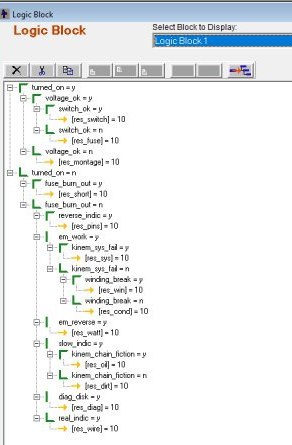
\includegraphics[width=\textwidth]{img/1}
	\caption{Оценки от полученных решений на плоскости критериев: красным выделено множество Парето}
\end{figure}  
Парето-оптимальными являются только решение Б1. С точки зрения ЛПР оно также является лучшим, так как позволяет достичь максимального дохода.

\section{Решение задачи стохастического программирования}
Рассмотрим задачу стохастического программирования на основе задачи однокритериальной оптимизации, которая была получена из исходной методом введения метрики в пространстве критериев (п. 1.3.6).

Преобразуем третье ограничение системы:
\begin{center}
$2x_{11}+2x_{12}+7*x_{21}+7*x_{22} \leq 1200$
\end{center}

 в вероятностное, тогда:
\begin{center}
$P(\alpha_{11}x_{11}+\alpha_{12}x_{12}+\alpha_{21}x_{21}+\alpha_{22}x_{22} \leq 1200)\geq \alpha$
\end{center}
где все $a_{ij}$ нормально распределены и имеют следующие математические ожидания и дисперсии:
\begin{center}
$M(\alpha_{11})=2, M(\alpha_{12})=2, M(\alpha_{21})=7, M(\alpha_{22})=7$
$D(\alpha_{11})=1, D(\alpha_{12})=1, D(\alpha_{21})=3.5, D(\alpha_{22})=3.5$
\end{center}
Где СКО равно половине математического ожидания. По таблице функции распределения стандартного нормального закона  находим $K_a (0.1\leq \alpha\leq 0.9)$
\begin{center}
$K_{0.1}=-1.2816, K_{0.2}=-0.8416, K_{0.3}=-0.5244, K_{0.4}=-0.2533, K_{0.5}=0$
$K_{0.6}=0.2533, K_{0.7}=0.5244, K_{0.8}=0.8416, K_{0.9}=1.2816$
\end{center}
Таким образом, вероятностное ограничение становится эквивалентно детерминированному неравенству:	
\begin{equation}
2x_{11}+2x_{12}+7*x_{21}+7*x_{22}+K_{\alpha}*\sqrt{x_{11}^2+x_{12}^2+3.5*x_{21}^2+3.5*x_{22}^2} \leq 1200
\end{equation}



Решение задачи представлено как скрипт в программе Matlab
\begin{lstlisting}[language={matlab}, caption={Решение задачи стохастического программирования}]
clc; clearvars
% Параметры
Tmin1 = (18*60)*0.7;  %Минимально допустимое время работы 1 станка
Tmin2 = (20*60)*0.7;  %Минимально допустимое время работы 2 станка
Tmax1 = (18*60);  %Максимально допустимое время работы 1 станка
Tmax2 = (20*60);  %Максимально допустимое время работы 2 станка

% Целевые функции
f1 = @(X) 30*X(1) + 20*X(3); % -> max
f2 = @(X) 3*(X(1)+X(2))+12*(X(3)+X(4)); % -> min
f3 = @(X) 45*X(2) + 21*X(4); % -> max
z1 = @(N) -f1(N); % -> min
z3 = @(N) -f3(N); % -> min

% Обобщенный критерий
z1_opt = -9160;
f2_opt = 1814.4;
z3_opt = -12804;

f = @(N) (1-z1(N)/z1_opt)^2+(1-f2(N)/f2_opt)^2+(1-z3(N)/z3_opt)^2;
% Функциональные ограничения
A = [
    1,1,5,5;
    -1,-1,-5,-5;
    -2,-2,-7,-7;
    1,1,0,0;
    0,0,1,1];
b = [Tmax1;-Tmin1;  -Tmin2;  5000; 9000];
Aeq = [];
beq = [];
% Параметрические ограничения
lb = [0; 0; 0; 0];
ub = [5000; 5000; 9000; 9000];
% Опции оптимизатора
options = optimoptions('fmincon','Display','none');
startingPoint = [0, 0, 0, 0];
% Параметры для задачи стохастического программирования
alpha = 0.1:0.1:0.9;
Ka = icdf('Normal', alpha, 0, 1); % Квантили распределения N(0,1)
global K
global m1; global m2; global m3; global m4
global d1; global d2; global d3; global d4
m1=2;m2=2;m3=7;m4=7;
d1=1;d2=1;d3=3.5;d4=3.5;
% Решение детерминированной задачи:
[Ndet, ~] = fmincon(f, startingPoint,[2,2,7,7; A], [Tmax2; b], Aeq, beq, lb, ub, [], options);
% Решение стохастической задачи:
N = zeros(4,numel(alpha));
for i = 1:numel(alpha)
 K = Ka(i);
 [N(:,i), ~] = fmincon(f, startingPoint, ...
 A, b, Aeq, beq, lb, ub, @nonlin, options);
end
%% Вывод результатов
F1 = cellfun(f1, num2cell(N,1));
F2 = cellfun(f2, num2cell(N,1));
F3 = cellfun(f3, num2cell(N,1));
fprintf('alpha = %.1f, X_11 = %6.4f, X_12 = %6.4f, x_21 = %6.4f, x_22 = %6.3f, f1 = %.2f, f2 = %.0f, f3 = %.2f\n', ...
 [alpha; N(1,:); N(2,:); N(3,:); N(4,:); F1; F2; F3])
fprintf('Для детерминированных ограничений:\n')
fprintf('X_11 = %3.4f, X_12 = %3.4f, x_21 = %6.4f, x_22 = %6.3f, f1 = %.2f, f2 = %.0f, f3 = %.2f\n', ...
 Ndet(1), Ndet(2), Ndet(3), Ndet(4), f1(Ndet), f2(Ndet), f3(Ndet))
%% Функция, задающая нелинейные ограничения
function [c, ceq] = nonlin(N)
global K;
global m1; global m2; global m3; global m4
global d1; global d2; global d3; global d4
  c = m1*N(1)+m2*N(2) + m3*N(3)+m4*N(4) + K*sqrt(d1*N(1)^2 + d2*N(2)^2 + d3*N(3)^2 + d4*N(4)^2) - 1200;
 ceq = [];
end
\end{lstlisting}
\begin{lstlisting}[language={matlab}, caption={Результат выполнения}]
alpha = 0.1, X_11 = 271.4401, X_12 = 278.9110, x_21 = 41.1291, x_22 =  0.001, f1 = 8965.78, f2 = 2145, f3 = 12551.01
alpha = 0.2, X_11 = 271.4492, X_12 = 278.9046, x_21 = 41.1151, x_22 =  0.014, f1 = 8965.78, f2 = 2145, f3 = 12551.01
alpha = 0.3, X_11 = 271.4494, X_12 = 278.9048, x_21 = 41.1172, x_22 =  0.012, f1 = 8965.83, f2 = 2145, f3 = 12550.97
alpha = 0.4, X_11 = 155.5649, X_12 = 205.9867, x_21 = 78.8894, x_22 =  0.000, f1 = 6244.73, f2 = 2031, f3 = 9269.41
alpha = 0.5, X_11 = 83.7126, X_12 = 152.2874, x_21 = 103.9999, x_22 =  0.000, f1 = 4591.37, f2 = 1956, f3 = 6852.93
alpha = 0.6, X_11 = 63.7924, X_12 = 88.9527, x_21 = 74.5707, x_22 = 46.080, f1 = 3405.19, f2 = 1906, f3 = 4970.56
alpha = 0.7, X_11 = 27.7783, X_12 = 43.1165, x_21 = 73.8482, x_22 = 63.173, f1 = 2310.31, f2 = 1857, f3 = 3266.87
alpha = 0.8, X_11 = 0.0000, X_12 = 0.0000, x_21 = 74.3433, x_22 = 74.343, f1 = 1486.87, f2 = 1784, f3 = 1561.21
alpha = 0.9, X_11 = 0.0000, X_12 = 0.0000, x_21 = 70.9449, x_22 = 70.990, f1 = 1418.90, f2 = 1703, f3 = 1490.78 
Для детерминированных ограничений:
X_11 = 83.7126, X_12 = 152.2874, x_21 = 103.9999, x_22 =  0.000, f1 = 4591.37, f2 = 1956, f3 = 6852.93
\end{lstlisting}

\tabulinesep = 1mm
\begin{longtabu} to \textwidth {|X[ c , m ] |X[c , m ] | X[ c , m ]|X[ c , m ]|X[ c , m ]|X[ c , m ]|X[ c , m ]|X[ c , m ]|}\firsthline\hline
\textbf{$\alpha$}&\textbf{$x_{11}$}&\textbf{$x_{12}$}&\textbf{$x_{21}$}&\textbf{$x_{22}$}&\textbf{$f_1$}&\textbf{$f_2$}&\textbf{$f_3$}\\ \hline \endfirsthead
0.1&271.4401&278.9110&41.1291& 0.001&8965.78&2145&12551.01\\ \hline
0.2&271.4492&278.9046&41.1151& 0.014&8965.78&2145&12551.01\\ \hline
0.3&271.4494&278.9048&41.1172& 0.012&8965.83&2145&12550.97\\ \hline
0.4&155.5649&205.9867&78.8894& 0.000&6244.73&2031&9269.41\\ \hline
0.5&83.7126&152.2874&103.9999& 0.000&4591.37&1956&6852.93\\ \hline
0.6&63.7924&88.9527&74.5707&46.080&3405.19&1906&4970.56\\ \hline
0.7&27.7783&43.1165&73.8482&63.173&2310.31&1857&3266.87\\ \hline
0.8&0.0000&0.0000&74.3433&74.343&1486.87&1784&1561.21\\ \hline
0.9&0.0000&0.0000&70.9449&70.990&1418.90&1703&1490.78\\ \hline
\multicolumn{8}{|c|}{Решение задачи при детерминированных ограничениях}\\ \hline
-&83.7126&152.2874&103.9999& 0.000&4591.37&1956&6852.93\\ \hline
\end{longtabu}
Задача чувствительна к выбранному ограничению, т.к. для различных K получились разные результаты. 

Увеличение доверительной вероятности $\alpha$ приводит к ухудшению оценок получаемых решений по первому и второму критерию. При $\alpha = 0.5, K_{\alpha} = 0$в случае чего получается решение, совпадающее с решением задачи с детерминированными ограничениями. 

При $\alpha < 0.5$ квантиль приобретает отрицательное значение. За счет чего ограничения \textbf{ослабевают}(их выполнение становится менее важным), и например решение при $\alpha = 0.1$ практические совпадает с оптимум для первого и второго критерия одновременно, чего не удалось добиться в каких-либо методах оптимизации.

А при $\alpha > 0.5$ ограничения становяться более \textbf{жесткими}, что уменьшает общий доход.



%------------------------------------------------------------------------------

%\addcontentsline{toc}{section}{Список литературы}
%\bibliography{thesis}
%\bibliographystyle{ugost2008}

\end{document}
\chapter{Поиск оптимальной стратегии принятия решений с использованием марковских моделей}
\section{Постановка задачи}

\subsubsection{Вариант 16}

Ежедневно утром производится проверка дорогостоящей машины с целью выявления, находится ли она в исправном состоянии, требует мелкого ремонта или нуждается в серьезном ремонте. Обозначим эти состояния 0, 1, 2 соответственно. Если машина находится в совершенно исправном состоянии, то вероятность того, что она останется в таком же состоянии на начало следующего дня, равна р(0|0), вероятность того, что потребуется мелкий ремонт, равна р(1|0) и вероятность того, что возникает необходимость серьезного ремонта, равна р(2|0). В случае когда машина требует ремонта, фирма может прибегнуть к услугам двух ремонтных фирм, одна из которых (фирма F, гарантирующая качество ремонта) взимает плату М за мелкий ремонт и плату R за крупный. Вторая (фирма Т, не гарантирующая качества ремонта) взымает соответственно плату m и r, где m<М и r<R. Легко себе представить, что качество работ, производимых фирмой F, выше, чем у фирмы Т, что отражается значением вероятности полностью исправного состояния машины на начало следующего за ремонтом дня. Пусть решение d=1 определяет выбор фирмы F и решение d=2 — выбор фирмы Т. Обозначим через р(j | i, d) вероятность перехода машины в состояние j на следующем отрезке (j=0,1,2) при условии, что она находится в состоянии I на текущем отрезке (i=1,2) и принимается решение d(d=1,2).
\\\\
р (0 | 0) = 0.6 (машина осталась исправной)\\
р (1 | 0) = 0.3 (машина требует мелкого ремонта)\\
р (2 | 0) = 0.1 (машина требует крупного ремонта)\\\\
р (0 | 1, 1) = 0.9 [М = 14] (фирма F выполнила мелкий ремонт)\\
р (1 | 1, 1) = 0.1 (фирма F в процессе выполнения мелкого ремонта)\\
р (2 | 1, 1) = 0 (невозможное событие -- если выполнен крупный ремонт, то мелкий не нужен)\\
р (0 | 2, 1) = 0.6 [R = 21] (фирма F выполнила крупный ремонт)\\
р (1 | 2, 1) = 0.3 [R – M = 7] (фирма F выполнила мелкий ремонт, но надо доделать до крупного)\\
р (2 | 2, 1) = 0.1 (фирма F в процессе выполнения крупного ремонта)\\\\
р (0 | 1, 2) = 0.7 [m = 12] (фирма T выполнила мелкий ремонт)\\
р (1 | 1, 2) = 0.2 (фирма T в процессе выполнения мелкого ремонта)\\
р (2 | 1, 2) = 0 (невозможное событие -- если выполнен крупный ремонт, то мелкий не нужен)\\
р (0 | 2, 2) = 0.5 [r = 19] (фирма T выполнила крупный ремонт)\\
р (1 | 2, 2) = 0.4 [r – m = 7] (фирма T выполнила мелкий ремонт, но надо доделать до крупного)\\
р (2 | 2, 2) = 0.1 (фирма T в процессе выполнения крупного ремонта)\\
\\
Найдите оптимальную стратегию и минимальные затраты на отрезке N=$\infty$.

\subsubsection{Доп задание}

Предположите, что фирме F для выполнения крупного ремонта требуется 1 полный рабочий день, а фирме Т — 2 полных рабочих
дня. Считайте далее, что фирма — владелец машины несет потери в размере $c$ единиц за каждый день ее простоя. Покажите, как при этих условиях нужно изменить уравнения.

\section{Решение}

\subsection{Решения и стратегии}

Имеется три состояния машины:

\begin{itemize}
	\item 1 -- исправна;
	\item 2 -- легкая поломка (необходим мелкий ремонт);
	\item 3 -- серьезная поломка (необходим крупный ремонт);
\end{itemize}

Для данных состояний имеется три решения:

\begin{itemize}
	\item $X_1$ -- ничего не делать;
	\item $X_2$ -- выбрать фирму F;
	\item $X_3$ -- выбрать фирму T;
\end{itemize}

Таким образом, возможны следующие стратегии:

\begin{table}[h!]
	\centering
	\bgroup
	\captionsetup{singlelinecheck = false, format= hang, justification=raggedleft, font=footnotesize, labelsep=space}
	\caption{Возможные стратегии}
	\def\arraystretch{1}
	\begin{tabular}{ | m{0.3cm} | m{2.2cm} | m{2.8cm} | m{3.1cm} | }
		\hline
		№ & Исправна & Легкая поломка & Серьезная поломка \\ \hline
		1 & $X_1, (-)$ & $X_2, (F)$ & $X_3, (T)$ \\ \hline
		2 & $X_1, (-)$ & $X_2, (F)$ & $X_2, (F)$ \\ \hline
		3 & $X_1, (-)$ & $X_3, (T)$ & $X_3, (T)$ \\ \hline
		4 & $X_1, (-)$ & $X_3, (T)$ & $X_1, (F)$ \\
		\hline
	\end{tabular}
	\egroup
\end{table}

\subsection{Построение матриц переходных вероятностей и матриц расходов}

$P_1$ и $P_2$ -- матрицы переходных вероятностей для компаний $F$ и $T$ соответственно:
\\

$
P_1=\begin{bmatrix}
0.6 & 0.3 & 0.1 \\
- & - & - \\
- & - & - \\
\end{bmatrix}
$
$
P_2=\begin{bmatrix}
- & - & - \\
0.9 & 0.1 & 0 \\
0.6 & 0.3 & 0.1 \\
\end{bmatrix}
$
$
P_3=\begin{bmatrix}
- & - & - \\
0.7 & 0.2 & 0.1 \\
0.5 & 0.4 & 0.1 \\
\end{bmatrix}
$\\

$R_1$ и $R_2$ -- матрицы расходов для компаний $F$ и $T$ соответственно:
\\

$
R_1=\begin{bmatrix}
0 & 0 & 0 \\
- & - & - \\
- & - & - \\
\end{bmatrix}
$
$
R_2=\begin{bmatrix}
- & - & - \\
14 & 0 & 0 \\
21 & 7 & 0 \\
\end{bmatrix}
$
$
R_3=\begin{bmatrix}
- & - & - \\
12 & 0 & 0 \\
19 & 7 & 0 \\
\end{bmatrix}
$\\

\subsection{Нахождение величин ожидаемого дохода}

Ожидаемый доход вычисляется по формуле:\\

$\nu_i(X_{k})=\sum_{j=1}^{m}p_{i,j}(X_{k})r_{i,j}(X_{k})$\\

Тогда для первого решения (ничего не делать):\\

$\nu_1(X_1)=0$

$\nu_2(X_1)=-$

$\nu_3(X_1)=-$\\

Для второго решения (выбрать фирму F):\\

$\nu_1(X_2)=-$

$\nu_2(X_2)=0.9\cdot 14=12.6$

$\nu_3(X_2)=0.6\cdot 21+0.3\cdot 7=14.7$\\

Тогда для третьего решения (выбрать фирму T):\\

$\nu_1(X_3)=-$

$\nu_2(X_3)=0.7\cdot 12=8.4$

$\nu_3(X_3)=0.5\cdot 19+0.4\cdot 7=12.3$\\

\subsection{Формулировка задачи в виде задачи линейного программирования}

Приведение к задаче линейного программирования производится следующим образом:

\begin{figure}[h!]
	\centering
	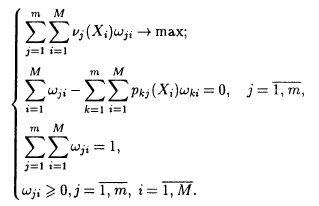
\includegraphics[scale = 0.90]{images/p2_1.png}
	\label{image:p2_1}
\end{figure}

Для данной задачи:

\begin{equation*}
\begin{cases}
\text{$0\cdot w_{11}+12.6\cdot w_{22}+8.4\cdot w_{23}+14.7\cdot w_{32}+12.3\cdot w_{33}\rightarrow min$} \\
\text{$(1-0.6)\cdot w_{11}-0.9\cdot w_{22}-0.7\cdot w_{23}-0.6\cdot w_{32}-0.5\cdot w_{33}=0$} \\
\text{$-0.3\cdot w_{11}+(1-0.1)\cdot w_{22}+(1-0.2)\cdot w_{23}-0.3\cdot w_{32}-0.4\cdot w_{33}=0$} \\
\text{$-0.1\cdot w_{11}-0\cdot w_{22}-0.1\cdot w_{23}+(1-0.1)\cdot w_{32}+(1-0.1)\cdot w_{33}=0$} \\
\text{$w_{11}+w_{22}+w_{23}+w_{32}+w_{33}=1$}
\text{$w_{ij}\geq 0, i=\overline{1,2,3}, j=\overline{1,2,3}$}
\end{cases}
\end{equation*}

\subsection{Решение задачи}

Разработаем скрипт для расчета вероятностей $w_{ij}$ в среде MATLAB (Приложение 9).

Результат расчета вероятностей:

\lstinputlisting{listings/p2.l1.log}

Таким образом машина исправна с вероятностью 61.82\%. Для мелкого ремонта следует обращаться в фирму T (28.18\%). Для крупного ремонта следует обращаться в фирму F (10\%).

\subsection{Дополнительное задание}

Предположите, что фирме F для выполнения крупного ремонта требуется 1 полный рабочий день, а фирме Т — 2 полных рабочих
дня. Считайте далее, что фирма — владелец машины несет потери в размере $c$ единиц за каждый день ее простоя. Покажите, как при этих условиях нужно изменить уравнения.

Для решения задачи нет смысла определять новые состояния, как это указано в методических указаниях. Достаточно просто изменить матрицы расходов для компаний $F$ и $T$ следующим образом:\\

$
R_1=\begin{bmatrix}
0 & 0 & 0 \\
- & - & - \\
- & - & - \\
\end{bmatrix}
$
$
R_2=\begin{bmatrix}
- & - & - \\
14 & 0 & 0 \\
21 + c & 7 + c & 0 \\
\end{bmatrix}
$
$
R_3=\begin{bmatrix}
- & - & - \\
12 & 0 & 0 \\
19 + 2\cdot c & 7 + 2\cdot c & 0 \\
\end{bmatrix}
$\\

Дальше задача решается аналогичным образом.

\section{Вывод}

Были определены оптимальные стратегии для конкретной задачи. Машина исправна с вероятностью 61.82\%. Для мелкого ремонта следует обращаться в фирму T (28.18\%). Для крупного ремонта следует обращаться в фирму F (10\%).

Линейное программирование позволяет достаточно легко и быстро решать подобные задачи, однако требует некоторых предварительных преобразований перед использованием.
\chapter{Поиск оптимальных параметров сети систем массового обслуживания}
\section{Постановка задачи}
\textbf{Вариант:} задача 4, вариант 144.

\tabulinesep = 1mm
\begin{longtabu} to \textwidth {|X[c , m ] |X[4,c , m ] | X[c , m ]|X[c , m ]|X[c , m ]| X[c , m ]|X[4,c , m ]|}\firsthline\hline

№ вар&$Q=\{q_{ij}\}_{\begin{matrix}i=\overline{0,n}\\j=\overline{0,n}\end{matrix}}$&$ca_0$&$\lambda_0$&$L_r$&$\mu$&$\{cs_j\}$\\ \hline
144&$\begin{array}{c|c|c|c|c}0& 0.2& 0.3& 0.2& 0.3\\ \hline 0.1&0&0.2&0.6&0.1\\ \hline 0.6&0.2&0&0.1&0.1\\ \hline 0&0.5&0.1&0&0.4\\ \hline 0.5&0.3&0.1&0.1&0 \end{array}$&0.16&8&-&10&$\begin{array}{c|c|c|c}0.04& 0.04& 0.04& 0.04	\end{array}$\\ \hline
\end{longtabu}

Найти:
\begin{equation*}
min L(\mu)=\sum_{j=1}^{n}L_j
\end{equation*}
При условии:
\begin{equation*}
\sum_{j=1}^{n}\mu_j=\mu
\end{equation*}

\section{Решение}
Вычислим мощность $\mu > \mu_j^1, cs$ и $ca$ для каждой станции.

Скорость прихода задач в узел j: $\lambda_j=\lambda_{0j}+\sum_{i=0}^nq_{ij}\lambda_i, j=0, ..., n$
\begin{equation*}
Q =
 \begin{pmatrix}
  0& 0.2& 0.3& 0.2& 0.3 \\
  0.1&0&0.2&0.6&0.1 \\
  0.6&0.2&0&0.1&0.1  \\
  0&0.5&0.1&0&0.4 \\
  0.5&0.3&0.1&0.1&0
 \end{pmatrix}
\end{equation*}
$\lambda_0=8$\\
$\lambda_1=0.2\lambda_0+0\lambda_1+0.2\lambda_2+0.5\lambda_3+0.3\lambda_4$\\
$\lambda_2=0.3\lambda_0+0.2\lambda_1+0\lambda_2+0.1\lambda_3+0.1\lambda_4$\\
$\lambda_3=0.2\lambda_0+0.6\lambda_1+0.1\lambda_2+0\lambda_3+0.1\lambda_4$\\
$\lambda_4=0.3\lambda_0+0.1\lambda_1+0.1\lambda_2+0.4\lambda_3+0\lambda_4$
\begin{lstlisting}[language={matlab}, caption={Код Matlab}, basicstyle=\ttfamily]
A = [1 0 0 0 0;
 0.2 -1 0.2 0.5 0.3;
 0.3 0.2 -1 0.1 0.1;
 0.2 0.6 0.1 -1 0.1;
 0.3 0.1 0.1 0.4 -1];
b=[8; 0; 0; 0; 0];
lambdaj=A\b
\end{lstlisting}
\begin{lstlisting}[language={matlab}, caption={Результат}, basicstyle=\ttfamily]
lambdaj =
    8.0000
    9.1128
    5.7833
    8.3697
    7.2375
\end{lstlisting}
Проверим полученный результат:
\begin{lstlisting}[language={matlab}, caption={Проверка}, basicstyle=\ttfamily]
>> [ 0 0.1 0.6 0 0.5] * lambdaj

ans =
    8.0000 
\end{lstlisting}
Как и ожидалось, была получена $\lambda_0$.\\Вычислим $ca_j$. Для этого, сперва найдем все $\lambda_{ij}$, где $\lambda_{ij} = \lambda_i*q_{ij}$.
\begin{lstlisting}[language={matlab}, caption={Код Matlab}, basicstyle=\ttfamily]
N=5;
Q = [0 0.2 0.3 0.2 0.3;
 0.1 0 0.2 0.6 0.1;
 0.6 0.2 0 0.1 0.1;
 0 0.5 0.1 0 0.4;
 0.5 0.3 0.1 0.1 0];
lambdaij=[];
for i = 1:N
 for j = 1:N
 lambdaij(i,j) = lambdaj(i)*Q(i, j);
 end
end
 lambdaij
\end{lstlisting}
\begin{lstlisting}[language={matlab}, caption={Результат}, basicstyle=\ttfamily]
lambdaij =

         0    1.6000    2.4000    1.6000    2.4000
    0.9113         0    1.8226    5.4677    0.9113
    3.4700    1.1567         0    0.5783    0.5783
         0    4.1849    0.8370         0    3.3479
    3.6188    2.1713    0.7238    0.7238         0
\end{lstlisting}

\begin{equation*}
\lambda =
 \begin{pmatrix}
  0  &  1.6   & 2.4   & 1.6    &2.4 \\
  0.91&    0   & 1.82  &  5.47  &  0.91 \\
  3.47 &   1.16 &   0   & 0.58   & 0.58  \\
  0    &4.18    &0.84    &0       &3.35 \\
  3.62  &  2.17  &  0.72  &  0.72  &  0
 \end{pmatrix}
\end{equation*}
Решим уравнения по формулам:
\begin{equation*}
ca_j=\frac{\lambda_{0j}}{\lambda_j}ca_{0j}+\sum_{i=1}^{n}\frac{\lambda_{ij}}{\lambda_j}ca_{ij}=\sum_{i=0}^{n}\frac{\lambda_{ij}}{\lambda_j}ca_{ij}
\end{equation*}

\begin{equation*}
cd_{ij}=q_{ij}cd_{ij}+1-q_{ij}
\end{equation*}

\begin{lstlisting}[language={matlab}, caption={Код Matlab}, basicstyle=\ttfamily]
caA = 0;
 caB = [0 0 0 0 0];
for j = 1:N
 for i = 1:N
 caA(j,i) = lambdaij(i,j)/lambdaj(j)*Q(i, j);
 caB(j)=caB(j)+lambdaij(i,j)/lambdaj(j)*(1-Q(i,j));
 end
end
 caA = caA-eye(5);
 caA(1,:) = [1 0 0 0 0];
 caA;
 caA^-1;
 caB = -caB';
 caB(1)=0.49;
 caj = (caA^-1)*caB
\end{lstlisting}
\begin{lstlisting}[language={matlab}, caption={Результат}, basicstyle=\ttfamily]
caj =
    0.1600
    0.9486
    0.8902
    0.9461
    0.9049
\end{lstlisting}
Вычислим $L_j$ и $P_j$
\begin{equation*}
p_j=\frac{\lambda_j}{\mu_jm_j}
\end{equation*}
\begin{equation*}
L_j(\lambda_j, ca_j, \mu_j, cs_j)=\frac{(\frac{\lambda_j}{\mu_j})^2(ca_j+cs_j)*g(\lambda_j, ca_j, \mu_j, cs_j)}{2(1-\frac{\lambda_j}{\mu_j})}+\frac{\lambda_j}{\mu_j}
\end{equation*}
\begin{equation*}
PI_j(\mu_j)=-V_j\frac{\partial L_j(\mu_j)}{\partial(\mu_j)}
\end{equation*}
Где:
\begin{equation*}
\lambda_j=9.1128, ca_0=0.16, cs_1=0.04
\end{equation*}
Для этого был написан скрипт matlab.
\begin{lstlisting}[language={matlab}, caption={Код Matlab}, basicstyle=\ttfamily]
for i = 2:N
 [Lj(i-1), Pj(i-1)] = params(lambdaj(i), caj(i), m(i-1), cs(i-1));
end
 Lj
 Pj
 L = sum(Lj)

function [ fLj, fPj ] = params( fl, fca, fm, fcs )
 Lj = '(l/m)^2*(ca+csj)*exp(-2*(1-l/m)*(1-ca)^2/(3*(l/m)*(ca+csj)))/(2*(1-l/m))';
 syms m;
 syms l;
 syms ca;
 syms csj;
 fLj = subs(Lj,l, fl);
 fLj = subs(fLj,m, fm);
 fLj = subs(fLj,ca, fca);
 fLj = subs(fLj,csj, fcs);
 fLj = vpa(fLj);
 
 Pj = '-((l)/(l-m)^2)';
 fPj = subs(Pj,l, fl);
 fPj = subs(fPj,m, fm);
 fPj = -1*vpa(fPj);
 end
\end{lstlisting}
\begin{lstlisting}[language={matlab}, caption={Результат}, basicstyle=\ttfamily]
Lj =
[ 4.6255839976370720273840674915939, 0.36659806895060537891974885952995, 2.1179331569743248761799734854413, 0.89370855816402942385738205100272]
 
 
Pj =
[ 11.576845733984487216317150244183, 0.32525589689516798523377343071108, 3.1492188330322032096928472738867, 0.94838805064508015837789082867662] 

L = 
8.0038237817260317063411718875679
\end{lstlisting}
Воспользуемся следующей формулой:
\begin{equation*}
PI_j(\mu_j,(\lambda_j+\varepsilon_j))=max\{PI_j(\mu_j), j\in J_0\}
\end{equation*}
Чем выше загрузка узла $J$, тем больше $PI_j=-\frac{\partial L(\mu_j)}{\partial\mu_j}$\\
Для узла $\textbf{M/M/1}$ имеем $PI_j=-\frac{\partial L(\mu_j)}{\partial\mu_j}=\frac{\lambda_j}{(\lambda_j-\mu_j)^2}$.
Благодаря расчётам по этой формуле, можно понять в каких узла нужно увеличивать или уменьшать интенсивность входного потока.\\
Далее, применим следующий алгоритм:
\begin{figure}[H]
  \centering
  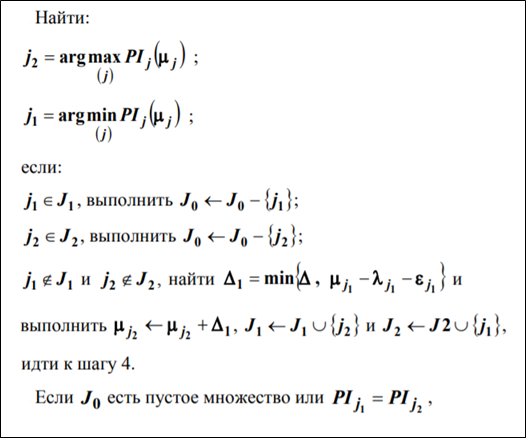
\includegraphics[width=.8\textwidth]{img/alg}
\end{figure}
Как значение $\Delta$ возьмем 0.5.\\По приведенному выше алгоритму определяем множества $J_0, J_1, J_2$. Результаты приведены в таблице \ref{tbl_1}.


\tabulinesep = 1mm
\begin{longtabu} to \textwidth {|X[ c , m ] |X[c , m ] | X[ c , m ]|X[ c , m ]|X[ c , m ]|}\firsthline\hline
№&$J_0$&$J_1$&$J_2$&Действия\\ \hline 
1&1,2,3,4&-&-&$\begin{array}{c} J_1 \leftarrow 1 \\ J_2 \leftarrow 2 \end{array}$ \\ \hline
2&1,2,3,4&1&2&$\begin{array}{c} J_1 \leftarrow 1 \\ J_2 \leftarrow 2 \end{array}$ \\ \hline
3&1,2,3,4&1&2&$\begin{array}{c} J_1 \leftarrow 3 \\ J_2 \leftarrow 2 \end{array}$ \\ \hline
4&1,2,3,4&1,3&2&$\begin{array}{c} J_1 \leftarrow 1 \\ J_2 \leftarrow 2 \end{array}$ \\ \hline
5&1,2,3,4&1,3&2&$\begin{array}{c} J_1 \leftarrow 3 \\ J_2 \leftarrow 4 \end{array}$ \\ \hline
6&1,2,3,4&1,3&2,4&$\begin{array}{c} J_1 \leftarrow 1 \\ J_2 \leftarrow 2 \end{array}$ \\ \hline
7&1,2,3,4&1,3&2,4&$\begin{array}{c} J_0 \leftarrow J_0-1\\ J_0 \leftarrow J_0-2\\ J_1 \leftarrow 2\\ J_2 \leftarrow 1 \end{array}$\\ \hline
8&3,4&1,2,3&1,2,4&$\begin{array}{c} J_1 \leftarrow 4 \\ J_2 \leftarrow 3 \end{array}$ \\ \hline
9&3,4&1,2,3,4&1,2,3,4&$\begin{array}{c} J_0 \leftarrow J_0-3\\ J_0 \leftarrow J_0-4\\ J_1 \leftarrow 3\\ J_2 \leftarrow 4 \end{array}$\\ \hline
10&-&1,2,3,4&1,2,3,4&- \\ \hline
\caption{Формирование множеств J}
\label{tbl_1}
\end{longtabu}
Результаты перераспределения мощностей представлено в таблице \ref{tbl_2}.

\tabulinesep = 1mm
\begin{longtabu} to \textwidth {|X[ c , m ] |X[c , m ] | X[ c , m ]|X[ c , m ]|X[ c , m ]| X[ c , m ]|}\firsthline\hline
№&$\mu_1$&$\mu_2$&$\mu_3$&$\mu_4$&Действия\\ \hline 
1&10&10&10&10&$\begin{array}{c} \mu_2-\Delta \\ \mu_1+\Delta  \end{array}$ \\ \hline
2&10.5&9.5&10&10&$\begin{array}{c} \mu_2-\Delta \\ \mu_1+\Delta  \end{array}$ \\ \hline
3&11&9&10&10&$\begin{array}{c} \mu_2-\Delta \\ \mu_3+\Delta  \end{array}$ \\ \hline
4&11&8.5&10.5&10&$\begin{array}{c} \mu_2-\Delta \\ \mu_1+\Delta  \end{array}$ \\ \hline
5&11.5&8&10.5&10&$\begin{array}{c} \mu_4-\Delta \\ \mu_3+\Delta  \end{array}$ \\ \hline
6&11.5&8&11&9.5&$\begin{array}{c} \mu_2-\Delta \\ \mu_1+\Delta  \end{array}$ \\ \hline
7&12&7.5&11&9.5&$\begin{array}{c} \mu_1-\Delta \\ \mu_2+\Delta  \end{array}$ \\ \hline
8&11.5&8&11&9.5&$\begin{array}{c} \mu_3-\Delta \\ \mu_4+\Delta  \end{array}$ \\ \hline
9&11.5&8&10.5&10&$\begin{array}{c} \mu_4-\Delta \\ \mu_3+\Delta  \end{array}$ \\ \hline
10&11.5&8&11&9.5&- \\ \hline
\caption{Перераспределение мощностей}
\label{tbl_2}
\end{longtabu}

Пересчитаем значения $PI_j, L_j$. Результаты вычисления $PI_j$ приведены в таблице \ref{tbl_3} и \ref{tbl_4}.

\tabulinesep = 1mm
\begin{longtabu} to \textwidth {|X[ c , m ] |X[c , m ] | X[ c , m ]|X[ c , m ]|X[ c , m ]|}\firsthline\hline
№&$PI_1$&$PI_2$&$PI_3$&$PI_4$\\ \hline 
1&	11.5768&0.3252&	3.1492&	0.9483\\ \hline 
2&	4.7354&	0.4186&	3.1492&	0.9483\\ \hline 
3&	2.5586&	0.5589&	3.1492&	0.9483\\ \hline 
4&	2.5586&	0.7835&	1.8443&	0.9483\\ \hline 
5&	1.5990&	1.1769&	1.8443&	0.9483\\ \hline 
6&	1.5990&	1.1769&	1.2098&	1.4138\\ \hline 
7&	1.0931&	1.9623&	1.2098&	1.4138\\ \hline 
8&	1.5990&	1.1769&	1.2098&	1.4138\\ \hline 
9&	1.5990&	1.1769&	1.8443&	0.9483\\ \hline 
10&	1.5990&	1.1769&	1.2098&	1.4138\\ \hline 

\caption{Пересчитанное $PI_j$}
\label{tbl_3}
\end{longtabu}


\tabulinesep = 1mm
\begin{longtabu} to \textwidth {|X[ c , m ] |X[c , m ] | X[ c , m ]|X[ c , m ]|X[ c , m ]| X[ c , m ]|}\firsthline\hline
№&	$L_1$&	$L_2$&	$L_3$&	$L_4$&	L\\ \hline 
1&	4.6255&	0.3665&	2.1179&	0.8937&	8.0038\\ \hline 
2&	2.8172&	0.4381&	2.1179&	0.8937&	6.2669\\ \hline 
3&	1.9765&	0.5347&	2.1179&	0.8937&	5.5229\\ \hline 
4&	1.9765&	0.6709&	1.5434&	0.8937&	5.0845\\ \hline 
5&	1.4944&	0.8743&	1.5434&	0.8937&	4.8059\\ \hline 
6&	1.4944&	0.8743&	1.1930&	1.1491&	4.7109\\ \hline 
7&	1.1840&	1.2051&	1.1930&	1.1491&	4.7313\\ \hline 
8&	1.4944&	0.8743&	1.1930&	1.1491&	4.7109\\ \hline 
9&	1.4944&	0.8743&	1.5434&	0.8937&	4.8059\\ \hline 
10&	1.4944&	0.8743&	1.1930&	1.1491&	4.7109\\ \hline 
\caption{Пересчитанное $L_j$ и $L$}
\label{tbl_4}
\end{longtabu}

\section{Вывод}
В данной работе была произведена оптимизация ССМО, в частности перераспределение мощностей в системе, для уменьшения очереди.\\\\
Начальные значения:\\
$\mu = (10, 10,10, 10)$\\
$L = 8.0038$\\
$L_j= (4.6255, 0.3655, 2.1179, 0.8937)$\\\\
После оптимизации:\\
$\mu = (10.5, 8, 11, 9.5)$\\
$L = 4.7109$\\
$L_j= (1.4944, 0.8743, 1.1930, 1.1491)$\\\\
Как и ожидалась, после оптимизации сети, загруженность системы понизилась.
\chapter{Решение задачи анализа потокового графа с использованием методики GERT и алгебры потоковых графов}
\section{Постановка задачи}
\textbf{Вариант:} 36.\\\\
\textbf{Дано:}
\begin{enumerate}
\item Граф GERT-сети
\begin{figure}[H]
  \centering
  \fbox{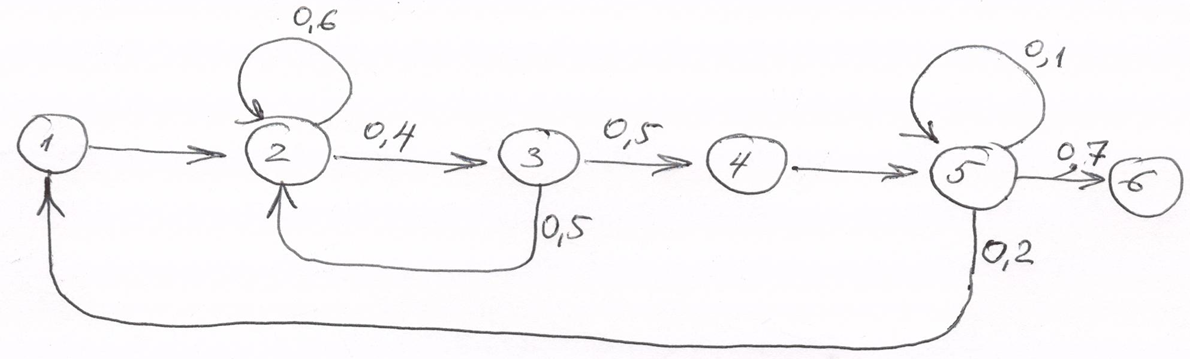
\includegraphics[width=.85\textwidth]{img/scheme_0}}
  \caption{Граф GERT-сети}
\end{figure}
\item Каждой дуге-работе ($ij$) поставлены в соответствие следующие данные:
\begin{enumerate}
\item Закон распределения времени выполнения работы. Будем считать его нормальным;
\item Параметры закона распределения (математическое ожидание \textbf{M} и дисперсия \textbf{D});
\item Вероятность $p_{ij}$ выполнения работы, показанная на графе.
\end{enumerate}
\end{enumerate}


\subsection{Задание}
\subsubsection{Часть 1}
Используя методику GERT, изложенную в книге «Методы анализа сетей»\\
Найти:
\begin{enumerate}
\item Вероятность выхода в завершающий узел графа (для всех вариантов узел 6);
\item Производящую функцию длительности процесса от начального узла  до завершающего узла;
\item Математическое ожидание длительности процесса от начального узла  до завершающего узла;
\item Дисперсию ожидание длительности процесса от начального узла  до завершающего узла;
\end{enumerate}
В отчете перечислить все петли всех порядков, обнаруженные на графе, выписать уравнение Мейсона, получить решение для $W_E(S)$ и найти требуемые параметры. Примерно так, как это сделано в примере на стр. 403–409 книги Филипса и Гарсиа «Методы анализа сетей»
\subsubsection{Часть 2}
Повторить пункты задания 2, 3, 4 используя методику анализа потокового графа, основанную на обработке матрицы передач (Branch Transmittance Matrix). 


Для выполнения задания рекомендуется пользоваться следующими источниками:
\begin{enumerate}
\item Филипс и Гарсиа «Методы анализа сетей»
\item Презентация GERT\_\&\_Flowgraph\_Algebra.pdf (выложена в ИНТРАНЕТ)
\item Ren\_The Methodology of Flowgraph.pdf
\end{enumerate}

\section{Решение}

\subsection{Часть 1}
Чтобы определить эквивалентную W-функцию для анализируемой GERT-сети, необходимо замкнуть сеть дугой, исходящей из узла 6 в узел 1 (рис. \ref{pic_1}).
\begin{figure}[H]
  \centering
  \fbox{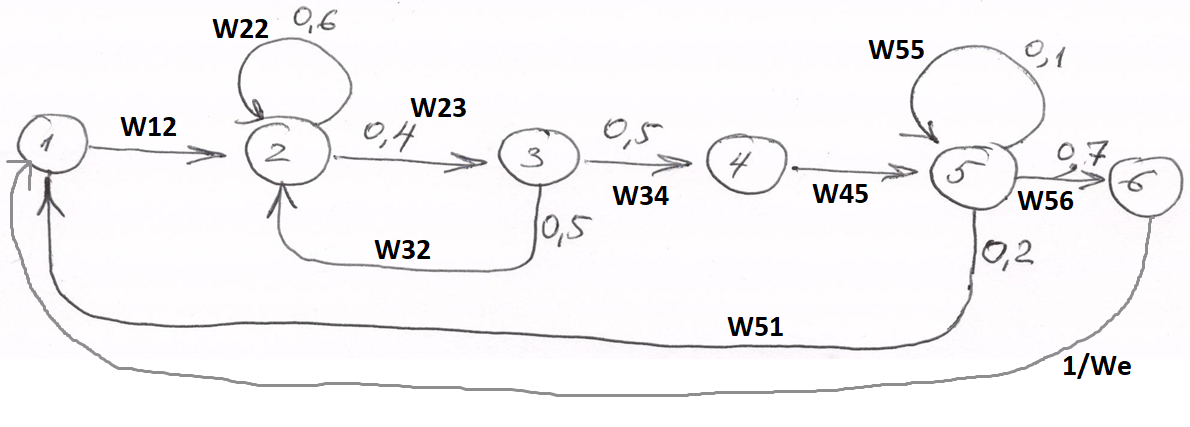
\includegraphics[width=\textwidth]{img/scheme_1}}
  \caption{Замкнутая GERT-сеть}
  \label{pic_1}
\end{figure}
Далее, выпишем в таблицу данные графа(мат. ожидание, дисперсия, W-функции)

\tabulinesep = 1mm
\begin{longtabu} to \textwidth {|X[8,c , m ] |X[8,c , m ] | X[15,l, m ]| X[15,l, m ]|X[15,l, m ]|X[25,l, m ]|}\firsthline\hline
\textbf{Начало}&\textbf{Конец}&\textbf{Вес ребра}&\textbf{Мат. ожидание}&\textbf{Дисперсия}&\textbf{W-функция}\\ \hline \endfirsthead
1	&2	&1	&20	&9	&$exp(20s+4.5s^2)$	\\ \hline
2	&2	&0.6&30	&16	&$0.6*exp(30s+8s^2)$	\\ \hline
2	&3	&0.4&40	&25	&$0.4*exp(40s+12.5s^2)$	\\ \hline
3	&2	&0.5&28	&16	&$0.5*exp(28s+8s^2)$	\\ \hline
3	&4	&0.5&37	&16	&$0.5*exp(37s+8s^2)$	\\ \hline
4	&5	&1	&30	&25	&$exp(30s+12.5s^2)$	\\ \hline
5	&1	&0.2&30	&16	&$0.2*exp(30s+8s^2)$	\\ \hline
5	&5	&0.1&10	&4	&$0.1*exp(10s+2s^2)$	\\ \hline
5	&6	&0.7&30	&16	&$0.7*exp(30s+8s^2)$	\\ \hline
\caption{Данные анализируемой GERT-сети}
\end{longtabu}
\textbf{Петли первого порядка:}
\begin{itemize}
\item $W_{12}W_{23}W_{34}W_{45}W_{51}$;
\item $W_{12}W_{23}W_{34}W_{45}W_{56}\frac{1}{W_e}$;
\item $W_{22}$;
\item $W_{23}W_{32}$;
\item $W_{55}$;
\end{itemize}
\textbf{Петли второго порядка:}
\begin{itemize}
\item $W_{22}W_{55}$;
\item $W_{55}W_{23}W_{32}$;
\end{itemize}
\textbf{Уравнение Мейсона}:
\begin{multline*}
H = 1 - W_{12}W_{23}W_{34}W_{45}W_{51} - W_{12}W_{23}W_{34}W_{45}W_{56}\frac{1}{W_e} - W_{22} - W_{23}W_{32} - W_{55}\\
 + W_{22}W_{55} + W_{55}W_{23}W_{32} = 0
\end{multline*}
\textbf{Выведем $W_E(S)$:}
\begin{equation*}
1 - W_{12}W_{23}W_{34}W_{45}W_{51} - W_{22} - W_{23}W_{32} - W_{55} + W_{22}W_{55} + W_{55}W_{23}W_{32} = W_{12}W_{23}W_{34}W_{45}W_{56}\frac{1}{W_e}
\end{equation*}
\begin{multline*}
W_E(S) =\\
(W_{12}W_{23}W_{34}W_{45}W_{56})/(1 - W_{12}W_{23}W_{34}W_{45}W_{51} - W_{22} - W_{23}W_{32} - W_{55} + W_{22}W_{55} + W_{55}W_{23}W_{32})
\end{multline*}

Вычислим математическое ожидание и дисперсию: $M_E(s) = 1$ при $s=0$

Так как $W_E(s)=p_E M_E (s)$,  то  $p_E=W_E(0)$, тогда $M_E(s)=\frac{W_E(s)}{p_E} =\frac{W_E(s)}{W_E(0)}$

Вычисляя первую и вторую производные по $s$ функции $M_E(s)$, и полагая $s=0$, находим математическое ожидание:
\begin{equation*}
\mu_{1E}=\frac{\partial M_E(s)}{\partial s}|s=0
\end{equation*}

и дисперсию:
\begin{equation*}
\sigma^2=\mu_{2E}-[\mu_{1E}]^2
\end{equation*}

Вероятность выхода в завершающий узел графа:
\begin{equation*}
p_E=W_E (0)
\end{equation*}
Для решения задачи был написан скрипт matlab, код приведен в приложении 4.

\begin{lstlisting}[language={matlab}, caption={Результат}, basicstyle=\ttfamily]
We =
-(7*exp((s*(91*s + 314))/2))/(5*exp(2*s*(s + 5)) - 3*exp(10*s*(s + 4)) + 30*exp(2*s*(4*s + 15)) - exp((3*s*(15*s + 52))/2) + 10*exp((s*(41*s + 136))/2) + 2*exp((s*(91*s + 314))/2) - 50)
 
We0 =
1
 
m1 =
2845/7
 
m2 =
11938987/49
 
D =
3844962/49
\end{lstlisting}
Были получены следующие результаты:
\begin{enumerate}
\item Вероятность выхода в завершающий узел графа равна 100\% ($p=W_E=1$).
\item Математическое ожидание 406,43.
\item Дисперсия времени выхода процесса в завершающий узел графа 78 468,61.
\end{enumerate}
\subsection{Часть 2}
Алгоритм дальнейших действий основан на:
\begin{itemize}
\item Презентация GERT\_\&\_Flowgraph\_Algebra.pdf (со слайда 56);
\item Ren\_The Methodology of Flowgraph.pdf (со страницы 35).
\end{itemize}
Определим матрицу Q, не забывая про обратную связь.
\begin{equation*}
Q = 
 \begin{pmatrix}
  0 & q_{12} & 0 & 0 & 0 & 0 \\
  0 & q_{22} & q_{23} & 0 & 0 & 0 \\ 
  0 & q_{32} & 0 & q_{34} & 0 & 0 \\ 
  0 & 0 & 0 & 0 & q_{45} & 0 \\ 
  q_{51} & 0 & 0 & 0 & q_{55} & q_{56} \\ 
  w_{61} & 0 & 0 & 0 & 0 & 0 
 \end{pmatrix}
\end{equation*}
Определим матрицу коэффициентов $A=I_6-Q^T$.
\begin{equation*}
A = 
 \begin{pmatrix}
    1&       0&    0&    0&    -q_{51}& -w_{61}\\
 -q_{12}& 1 - q_{22}& -q_{32}&    0&       0&    0\\
    0&    -q_{23}&    1&    0&       0&    0\\
    0&       0& -q_{34}&    1&       0&    0\\
    0&       0&    0& -q_{45}& 1 - q_{55}&    0\\
    0&       0&    0&    0&    -q_{56}&    1
 \end{pmatrix}
\end{equation*}
Находим 
\begin{equation*}
det(A)
\end{equation*}
далее
\begin{equation*}
\frac{\partial det(A)}{\partial w_{61}}
\end{equation*}
\begin{equation*}
det(A | w_{61}=0)
\end{equation*}
Далее можно вывести $W_E(S)$ с помощью формулы:
\begin{equation*}
W_E(S)=-\frac{\frac{\partial det(A)}{\partial w_{61}}}{det(A | w_{61}=0)}
\end{equation*}
Для расчетов, был написан matlab скрипт, код представлен в приложении 5.

\begin{lstlisting}[language={matlab}, caption={Результат}, basicstyle=\ttfamily]
[    1,       0,    0,    0,    -q51, -w61]
[ -q12, 1 - q22, -q32,    0,       0,    0]
[    0,    -q23,    1,    0,       0,    0]
[    0,       0, -q34,    1,       0,    0]
[    0,       0,    0, -q45, 1 - q55,    0]
[    0,       0,    0,    0,    -q56,    1]
 
 
-(q12*q23*q34*q45*q56)/(q22 + q55 + q23*q32 - q22*q55 - q23*q32*q55 + q12*q23*q34*q45*q51 - 1)
\end{lstlisting}
Во второй строчке был получен $W_E(S)$, который полностью(за исключением знаков) совпадает с $W_E(S)$ найденным в части 1.

Далее, имея $W_E(S)$ находим необходимые переменные.

Для расчетов, был использован скрипт из приложения 6.

\begin{lstlisting}[language={matlab}, caption={Результат}, basicstyle=\ttfamily]
We =
-(7*exp((s*(91*s + 314))/2))/(5*exp(2*s*(s + 5)) - 3*exp(10*s*(s + 4)) + 30*exp(2*s*(4*s + 15)) - exp((3*s*(15*s + 52))/2) + 10*exp((s*(41*s + 136))/2) + 2*exp((s*(91*s + 314))/2) - 50)
 
We0 =
1
 
m1 =
2845/7
 
m2 =
11938987/49
 
D =
3844962/49
\end{lstlisting}
Были получены следующие результаты:
\begin{enumerate}
\item Вероятность выхода в завершающий узел графа равна 100\% ($p=W_E=1$).
\item Математическое ожидание 406,43.
\item Дисперсия времени выхода процесса в завершающий узел графа 78 468,61.
\end{enumerate}
Которые полностью совпадает с результатами части 1.

\addcontentsline{toc}{chapter}{Заключение}
\chapter*{Заключение}
В работе были рассмотрены различные математические модели для решения задачи выбора оптимального решения.

При анализе результатов решения многокритериальной задачи можно заметить, что аддитивная и мультипликативная свертка выдают одинаковый, наиболее оптимальный результат. Наилучший результат этих методов обусловлен наличием коэффициентов значимости. Методы, не подразумевающие введение весовых коэффициентов показывают похожий результат, который в целом хуже, чем у аддитивной и мультипликативной свертки.

В процессе поиска оптимальной стратегии принятия решений с использованием марковских моделей были определены оптимальные стратегии для конкретной задачи. Линейное программирование позволяет достаточно легко и быстро находить оптимальную стратегию, однако требует некоторых предварительных преобразований и формализаций перед использованием.

Как и ожидалось, при оптимизации многоканальной замкнутой ССМО алгоритм простых итераций не сходится, поэтому пришлось использовать более надежный алгоритм Ньютона. Модифицированный алгоритм Ньютона чрезвычайно чувствителен к выбору начального приближения, поэтому был использован вариант алгоритма с расчетом матрицы Якоби. Для увеличения производительности данного алгоритма можно подключить пакет MATLAB Parallel Computing Toolbox, который использует MPI для эффективного распараллеливания.

В результате решения задачи анализа потокового графа можно сделать вывод, что при  заданных значениях вероятности, мат. ожидания и дисперсии для каждой дуги исходного графа достаточно легко расчитываются W-функции, которые необходимы для построения формулы Мейсона. После этого из формулы Мейсона по формулам математической статистики достаточно легко расчитывается результирующее мат. ожидание и дисперсия. Решение путем анализа потокового графа показало аналогичные результаты, что подтверждает корректность решения. Однако, метод анализа потокового графа выполняется заметно медленнее, даже на небольшом графе.

Среда MATLAB действительно хорошо подходит для решения оптимизационных задач засчет множества специфичных математических библиотек и пакетов.

%------------------------------------------------------------------------------

%\addcontentsline{toc}{section}{Список литературы}
%\bibliography{thesis}
%\bibliographystyle{ugost2008}

%\nocite{phill}
%\nocite{Ren}

\addcontentsline{toc}{chapter}{Список использованных источников}
\chapter*{Список использованных источников}
\begin{enumerate}
\item Д. Филлипс, А. Гарсиа-Диас. Методы анализа сетей: Пер. с англ. — М.: Мир, 1984.—496 с, ил.
\item Ren, Yu. The methodology of flowgraph models. PhD thesis, The London School of Economics and Political Science (LSE). –– 2011.
\item Сиднев А. Г. Системный анализ. Часть 1 [Электронный ресурс] // Интранет-
портал ИИТУ СПбПУ. 2018. URL: http://intranet.ftk.spbstu.ru/docinfo.php?InfoFtkDocumentID= 1386947 (дата обращения: 22.04.2018)
\item Горбунов В.М. Теория принятия решений: учебное пособие. Томск: Изд-во
Томск. политех. ун-та, 2010.
\item Системный анализ и принятие решений: учебное пособие / Е.Н. Бендерская,
Д.Н. Колесников, В.И. Пахомова и др.; Под ред. Д.Н. Колесникова. 2-е изд.
СПб.: Изд-во СПбГПУ, 2001.
\item Optimization Toolbox: описание функции FGOALATTAIN [Электронный ре-
сурс] // MATLAB.Exponenta, центр компетенций MathWorks. URL:
http://matlab.exponenta.ru/ optimiz/book\_4/2/fgoalattain.php (дата обращения:
17.02.2018).
\item Таха Х. А. Введение в исследование операций: Пер. с англ. 7-е изд. М.: Изда-тельский дом «Вильямс», 2005.
\end{enumerate}


%\bibliography{thesis}
%\bibliographystyle{ugost2008}


\clearpage
\addcontentsline{toc}{chapter}{Приложения}
\setcounter{section}{0}
\section*{Приложение 1} \label{p1:1}
\textbf{Решение задачи методом линейного программирования}
\begin{lstlisting}[language={matlab}, caption={Решение задачи методом линейного программирования}, label={lst:0}, basicstyle={\footnotesize\ttfamily}, breaklines={true}]
clear all;
close all; 
clc;
format long g;

% -F1 -> min
mF1 = @(X) -(60 * X(1) + 300 * X(2) + 2000 * X(3));
% -F2 -> min
mF2 = @(X) -((0.1 * X(1) + 10 * X(2) + 70 * sqrt(X(3))) ^ 1.5);
% F3 -> min
pF3 = @(X) 30 * X(1) + 100 * X(2) + 220 * X(3);
% F4 -> min
pF4 = @(X) log(20 * X(1) + 3 * X(2) + 0.01 * X(3));
% -F5 -> min
mF5 = @(X) -((-mF1(X)) / (X(1) + X(2) + X(3)));
% -F6 -> min
mF6 = @(X) -(((-mF1(X)) + (-mF2(X))) - (pF3(X) + pF4(X)));

A = [1, 0, 0;
-1, 0, 0;
0, 1, 0;
0, -1, 0;
0, 0, 1;
0, 0, -1;
1, 1, 1];

B = [70;
-35;
30;
-15;
1;
-0.5;
80];

Aeq = [];
Beq = [];

S = [35; 15; 0.5];

[x1, result1] = fmincon(mF1, S, A, B, Aeq, Beq);
[x2, result2] = fmincon(mF2, S, A, B, Aeq, Beq);
[x3, result3] = fmincon(pF3, S, A, B, Aeq, Beq);
[x4, result4] = fmincon(pF4, S, A, B, Aeq, Beq);
[x5, result5] = fmincon(mF5, S, A, B, Aeq, Beq);
[x6, result6] = fmincon(mF6, S, A, B, Aeq, Beq);

formatter = '-- F1 max --\n%s\n%s\n\n-- F2 max --\n%s\n%s\n\n-- F3 min --\n%s\n%s\n\n-- F4 min --\n%s\n%s\n\n-- F5 max --\n%s\n%s\n\n-- F6 max --\n%s\n%s\n\n';
s1 = sprintf('x1 = %.3f, x2 = %.3f, x3 = %.3f, x1 + x2 + x3 = %.3f', x1, sum(x1));
s2 = sprintf('!F1 = %.3f, F2 = %.3f, F3 = %.3f, F4 = %.3f, F5 = %.3f, F6 = %.3f', -result1, -mF2(x1), pF3(x1), pF4(x1), -mF5(x1), -mF6(x1));
s3 = sprintf('x1 = %.3f, x2 = %.3f, x3 = %.3f, x1 + x2 + x3 = %.3f', x2, sum(x2));
s4 = sprintf('F1 = %.3f, !F2 = %.3f, F3 = %.3f, F4 = %.3f, F5 = %.3f, F6 = %.3f', -mF1(x2), -result2, pF3(x2), pF4(x2), -mF5(x2), -mF6(x2)); 
s5 = sprintf('x1 = %.3f, x2 = %.3f, x3 = %.3f, x1 + x2 + x3 = %.3f', x3, sum(x3));
s6 = sprintf('F1 = %.3f, F2 = %.3f, !F3 = %.3f, F4 = %.3f, F5 = %.3f, F6 = %.3f', -mF1(x3), -mF2(x3), result3, pF4(x3), -mF5(x3), -mF6(x3)); 
s7 = sprintf('x1 = %.3f, x2 = %.3f, x3 = %.3f, x1 + x2 + x3 = %.3f', x4, sum(x4));
s8 = sprintf('F1 = %.3f, F2 = %.3f, F3 = %.3f, !F4 = %.3f, F5 = %.3f, F6 = %.3f', -mF1(x4), -mF2(x4), pF3(x4), result4, -mF5(x4), -mF6(x4));
s9 = sprintf('x1 = %.3f, x2 = %.3f, x3 = %.3f, x1 + x2 + x3 = %.3f', x5, sum(x5));
s10 = sprintf('F1 = %.3f, F2 = %.3f, F3 = %.3f, F4 = %.3f, !F5 = %.3f, F6 = %.3f', -mF1(x5), -mF2(x5), pF3(x5), pF4(x5), -result5, -mF6(x5)); 
s11 = sprintf('x1 = %.3f, x2 = %.3f, x3 = %.3f, x1 + x2 + x3 = %.3f', x6, sum(x6));
s12 = sprintf('F1 = %.3f, F2 = %.3f, F3 = %.3f, F4 = %.3f, F5 = %.3f, !F6 = %.3f', -mF1(x6), -mF2(x6), pF3(x6), pF4(x6), -mF5(x6), -result6);
fprintf(formatter, s1, s2, s3, s4, s5, s6, s7, s8, s9, s10, s11, s12);
\end{lstlisting}

\section*{Приложение 2} \label{p1:2}
\textbf{Решение задачи при помощи аддитивной свертки}
\begin{lstlisting}[language={matlab}, caption={Решение задачи при помощи аддитивной свертки}, label={lst:0}, basicstyle={\footnotesize\ttfamily}, breaklines={true}]
clear all;
close all; 
clc;
format long g;

% -F1 -> min
mF1 = @(X) -(60 * X(1) + 300 * X(2) + 2000 * X(3));
% -F2 -> min
mF2 = @(X) -((0.1 * X(1) + 10 * X(2) + 70 * sqrt(X(3))) ^ 1.5);
% F3 -> min
pF3 = @(X) 30 * X(1) + 100 * X(2) + 220 * X(3);
% F4 -> min
pF4 = @(X) log(20 * X(1) + 3 * X(2) + 0.01 * X(3));
% -F5 -> min
mF5 = @(X) -((-mF1(X)) / (X(1) + X(2) + X(3)));
% -F6 -> min
mF6 = @(X) -(((-mF1(X)) + (-mF2(X))) - (pF3(X) + pF4(X)));

cF2 = 0.15;
rF2 = 7258.939;
cF3 = 0.15;
rF3 = 2660;
cF4 = 0.05;
rF4 = 6.613;
cF5 = 0.05;
rF5 = 198.485;
cF6 = 0.6;
rF6 = 16501.964;

pFS = @(X) cF2 * (mF2(X) / rF2) + cF3 * (pF3(X) / rF3) + cF4 * (pF4(X) / rF4) + cF5 * (mF5(X) / rF5) + cF6 * (mF6(X) / rF6);

A = [1, 0, 0;
-1, 0, 0;
0, 1, 0;
0, -1, 0;
0, 0, 1;
0, 0, -1;
1, 1, 1];

B = [70;
-35;
30;
-15;
1;
-0.5;
80];

Aeq = [];
Beq = [];

S = [35; 15; 0.5];

[xS, resultS] = fmincon(pFS, S, A, B, Aeq, Beq);

formatter = '-- FS --\n%s\n%s\n%s\n%s\n\n';
s1 = sprintf('FS = %.3f', resultS);
s2 = sprintf('x1 = %.3f, x2 = %.3f, x3 = %.3f, x1 + x2 + x3 = %.3f', xS, sum(xS));
s3 = sprintf('F2 = %.3f, F3 = %.3f, F4 = %.3f, F5 = %.3f, F6 = %.3f', -mF2(xS), pF3(xS), pF4(xS), -mF5(xS), -mF6(xS));
s4 = sprintf('F2/rF2 = %.3f%%, F3/rF3 = %.3f%%, F4/rF4 = %.3f%%, F5/rF5 = %.3f%%, F6/rF6 = %.3f%%', -mF2(xS) / rF2 * 100, pF3(xS) / rF3 * 100, pF4(xS) / rF4 * 100, -mF5(xS) / rF5 * 100, -mF6(xS) / rF6 * 100);
fprintf(formatter, s1, s2, s3, s4);
\end{lstlisting}

\section*{Приложение 3} \label{p1:3}
\textbf{Решение задачи при помощи мультипликативной свертки}
\begin{lstlisting}[language={matlab}, caption={Решение задачи при помощи мультипликативной свертки}, label={lst:0}, basicstyle={\footnotesize\ttfamily}, breaklines={true}]
clear all;
close all; 
clc;
format long g;

% 1 / F1 -> min
mF1 = @(X) 1 / (60 * X(1) + 300 * X(2) + 2000 * X(3));
% 1 / F2 -> min
mF2 = @(X) 1 / ((0.1 * X(1) + 10 * X(2) + 70 * sqrt(X(3))) ^ 1.5);
% F3 -> min
pF3 = @(X) 30 * X(1) + 100 * X(2) + 220 * X(3);
% F4 -> min
pF4 = @(X) log(20 * X(1) + 3 * X(2) + 0.01 * X(3));
% 1 / F5 -> min
mF5 = @(X) 1 / ((1 / mF1(X)) / (X(1) + X(2) + X(3)));
% 1 / F6 -> min
mF6 = @(X) 1 / (((1 / mF1(X)) + (1 / mF2(X))) - (pF3(X) + pF4(X)));

cF2 = 0.15;
rF2 = 7258.939;
cF3 = 0.15;
rF3 = 2660;
cF4 = 0.05;
rF4 = 6.613;
cF5 = 0.05;
rF5 = 198.485;
cF6 = 0.6;
rF6 = 16501.964;

pFS = @(X) nthroot(mF2(X) * rF2, 1 / cF2) * nthroot(pF3(X) / rF3, 1 / cF3) * nthroot(pF4(X) / rF4, 1 / cF4) * nthroot(mF5(X) * rF5, 1 / cF5) * nthroot(mF6(X) * rF6, 1 / cF6);

A = [1, 0, 0;
-1, 0, 0;
0, 1, 0;
0, -1, 0;
0, 0, 1;
0, 0, -1;
1, 1, 1];

B = [70;
-35;
30;
-15;
1;
-0.5;
80];

Aeq = [];
Beq = [];

S = [35; 15; 0.5];

[xS, resultS] = fmincon(pFS, S, A, B, Aeq, Beq);

formatter = '-- FS --\n%s\n%s\n%s\n%s\n\n';
s1 = sprintf('FS = %.3f', resultS);
s2 = sprintf('x1 = %.3f, x2 = %.3f, x3 = %.3f, x1 + x2 + x3 = %.3f', xS, sum(xS));
s3 = sprintf('F2 = %.3f, F3 = %.3f, F4 = %.3f, F5 = %.3f, F6 = %.3f', 1 / mF2(xS), pF3(xS), pF4(xS), 1 / mF5(xS), 1 / mF6(xS));
s4 = sprintf('F2/rF2 = %.3f%%, F3/rF3 = %.3f%%, F4/rF4 = %.3f%%, F5/rF5 = %.3f%%, F6/rF6 = %.3f%%', (1 / mF2(xS)) / rF2 * 100, pF3(xS) / rF3 * 100, pF4(xS) / rF4 * 100, (1 / mF5(xS)) / rF5 * 100, (1 / mF6(xS)) / rF6 * 100);
fprintf(formatter, s1, s2, s3, s4);
\end{lstlisting}

\section*{Приложение 4} \label{p1:4}
\textbf{Решение задачи при помощи функции fminimax}
\begin{lstlisting}[language={matlab}, caption={Решение задачи при помощи функции fminimax}, label={lst:0}, basicstyle={\footnotesize\ttfamily}, breaklines={true}]
clear all;
close all; 
clc;
format long g;

% 1 / F1 -> min
mF1 = @(X) 1 / (60 * X(1) + 300 * X(2) + 2000 * X(3));
% 1 / F2 -> min
mF2 = @(X) 1 / ((0.1 * X(1) + 10 * X(2) + 70 * sqrt(X(3))) ^ 1.5);
% F3 -> min
pF3 = @(X) 30 * X(1) + 100 * X(2) + 220 * X(3);
% F4 -> min
pF4 = @(X) log(20 * X(1) + 3 * X(2) + 0.01 * X(3));
% 1 / F5 -> min
mF5 = @(X) 1 / ((1 / mF1(X)) / (X(1) + X(2) + X(3)));
% 1 / F6 -> min
mF6 = @(X) 1 / (((1 / mF1(X)) + (1 / mF2(X))) - (pF3(X) + pF4(X)));

rF1 = 13940;
rF2 = 7258.939;
rF3 = 2660;
rF4 = 6.613;
rF5 = 198.485;
rF6 = 16501.964;

A = [1, 0, 0;
-1, 0, 0;
0, 1, 0;
0, -1, 0;
0, 0, 1;
0, 0, -1;
1, 1, 1];

B = [70;
-35;
30;
-15;
1;
-0.5;
80];

Aeq = [];
Beq = [];

S = [35; 15; 0.5];

[xS, resultS] = fminimax(@m4f, S, A, B, Aeq, Beq);

formatter = '-- FS --\n%s\n%s\n%s\n%s\n\n';
s1 = sprintf('FS = (%.3f, %.3f, %.3f, %.3f, %.3f)', resultS(2:6));
s2 = sprintf('x1 = %.3f, x2 = %.3f, x3 = %.3f, x1 + x2 + x3 = %.3f', xS, sum(xS));
s3 = sprintf('F2 = %.3f, F3 = %.3f, F4 = %.3f, F5 = %.3f, F6 = %.3f', 1 / mF2(xS), pF3(xS), pF4(xS), 1 / mF5(xS), 1 / mF6(xS));
s4 = sprintf('F2/rF2 = %.3f%%, F3/rF3 = %.3f%%, F4/rF4 = %.3f%%, F5/rF5 = %.3f%%, F6/rF6 = %.3f%%', (1 / mF2(xS)) / rF2 * 100, pF3(xS) / rF3 * 100, pF4(xS) / rF4 * 100, (1 / mF5(xS)) / rF5 * 100, (1 / mF6(xS)) / rF6 * 100);
fprintf(formatter, s1, s2, s3, s4);
\end{lstlisting}

\begin{lstlisting}[language={matlab}, caption={Внутренняя функция для fminimax}, label={lst:0}, basicstyle={\footnotesize\ttfamily}, breaklines={true}]
function result = m4f(X)
	% 1 / F1 -> min
	mF1 = 1 / (60 * X(1) + 300 * X(2) + 2000 * X(3));
	% 1 / F2 -> min
	mF2 = 1 / ((0.1 * X(1) + 10 * X(2) + 70 * sqrt(X(3))) ^ 1.5);
	% F3 -> min
	pF3 = 30 * X(1) + 100 * X(2) + 220 * X(3);
	% F4 -> min
	pF4 = log(20 * X(1) + 3 * X(2) + 0.01 * X(3));
	% 1 / F5 -> min
	mF5 = 1 / ((1 / mF1) / (X(1) + X(2) + X(3)));
	% 1 / F6 -> min
	mF6 = 1 / (((1 / mF1) + (1 / mF2)) - (pF3 + pF4));
	
	rF1 = 13940;
	rF2 = 7258.939;
	rF3 = 2660;
	rF4 = 6.613;
	rF5 = 198.485;
	rF6 = 16501.964;
	
	result(1) = mF1 * rF1;
	result(2) = mF2 * rF2;
	result(3) = pF3 / rF3;
	result(4) = pF4 / rF4;
	result(5) = mF5 * rF5;
	result(6) = mF6 * rF6;
end
\end{lstlisting}

\section*{Приложение 5} \label{p1:5}
\textbf{Решение задачи при помощи метода последовательных уступок}
\begin{lstlisting}[language={matlab}, caption={Решение задачи для критерия F7}, label={lst:0}, basicstyle={\footnotesize\ttfamily}, breaklines={true}]
clear all;
close all; 
clc;
format long g;

% -F7 -> min
mF7 = @(X) -(30 * X(1) + 200 * X(2) + 1780 * X(3));
% -F8 -> min
mF8 = @(X) -(X(1) + 10 * X(3));
% F9 -> min
pF9 = @(X) X(1) + 2 * X(2);

A = [1, 0, 0;
-1, 0, 0;
0, 1, 0;
0, -1, 0;
0, 0, 1;
0, 0, -1;
1, 1, 1];

B = [70;
-35;
30;
-15;
1;
-0.5;
80];

Aeq = [];
Beq = [];

S = [35; 15; 0.5];

[x7, result7] = fmincon(mF7, S, A, B, Aeq, Beq);

formatter = '-- F7 max --\n%s\n%s\n\n';
s1 = sprintf('x1 = %.3f, x2 = %.3f, x3 = %.3f, x1 + x2 + x3 = %.3f', x7, sum(x7));
s2 = sprintf('!F7 = %.3f, F8 = %.3f, F9 = %.3f', -result7, -mF8(x7), pF9(x7)); 
fprintf(formatter, s1, s2);
\end{lstlisting}

\begin{lstlisting}[language={matlab}, caption={Решение задачи для критерия F8}, label={lst:0}, basicstyle={\footnotesize\ttfamily}, breaklines={true}]
clear all;
close all; 
clc;
format long g;

% -F7 -> min
mF7 = @(X) -(30 * X(1) + 200 * X(2) + 1780 * X(3));
% -F8 -> min
mF8 = @(X) -(X(1) + 10 * X(3));
% F9 -> min
pF9 = @(X) X(1) + 2 * X(2);

K = 0.85

rF7 = 9250;

A = [1, 0, 0;
-1, 0, 0;
0, 1, 0;
0, -1, 0;
0, 0, 1;
0, 0, -1;
1, 1, 1;
-30, -200, -1780];

B = [70;
-35;
30;
-15;
1;
-0.5;
80;
-rF7 * K];

Aeq = [];
Beq = [];

S = [35; 15; 0.5];

[x8, result8] = fmincon(mF8, S, A, B, Aeq, Beq);

fprintf('%.3f >= F7 >= %.1f * %.3f\n', rF7, K, rF7);
fprintf('%.3f >= F7 >= %.3f\n\n', rF7, rF7 * K);

formatter = '-- F8 max --\n%s\n%s\n\n';
s1 = sprintf('x1 = %.3f, x2 = %.3f, x3 = %.3f, x1 + x2 + x3 = %.3f', x8, sum(x8));
s2 = sprintf('F7 = %.3f, !F8 = %.3f, F9 = %.3f', -mF7(x8), -result8, pF9(x8)); 
fprintf(formatter, s1, s2);
\end{lstlisting}

\begin{lstlisting}[language={matlab}, caption={Решение задачи для критерия F9}, label={lst:0}, basicstyle={\footnotesize\ttfamily}, breaklines={true}]
clear all;
close all; 
clc;
format long g;

% -F7 -> min
mF7 = @(X) -(30 * X(1) + 200 * X(2) + 1780 * X(3));
% -F8 -> min
mF8 = @(X) -(X(1) + 10 * X(3));
% F9 -> min
pF9 = @(X) X(1) + 2 * X(2);

K = 0.85

rF7 = 9250;
rF8 = 67.162;

A = [1, 0, 0;
-1, 0, 0;
0, 1, 0;
0, -1, 0;
0, 0, 1;
0, 0, -1;
1, 1, 1;
-30, -200, -1780;
-1, 0, -10];

B = [70;
-35;
30;
-15;
1;
-0.5;
80;
-rF7 * K;
-rF8 * K];

Aeq = [];
Beq = [];

S = [35; 15; 0.5];

[x9, result9] = fmincon(pF9, S, A, B, Aeq, Beq);

fprintf('%.3f >= F7 >= %.2f * %.3f\n', rF7, K, rF7);
fprintf('%.3f >= F7 >= %.3f\n\n', rF7, rF7 * K);

fprintf('%.3f >= F8 >= %.2f * %.3f\n', rF8, K, rF8);
fprintf('%.3f >= F8 >= %.3f\n\n', rF8, rF8 * K);

formatter = '-- F9 max --\n%s\n%s\n\n';
s1 = sprintf('x1 = %.3f, x2 = %.3f, x3 = %.3f, x1 + x2 + x3 = %.3f', x9, sum(x9));
s2 = sprintf('F7 = %.3f, F8 = %.3f, !F9 = %.3f', -mF7(x9), -mF8(x9), result9); 
fprintf(formatter, s1, s2);
\end{lstlisting}

\section*{Приложение 6} \label{p1:6}
\textbf{Решение задачи при помощи метода достижения цели (fgoalattain)}
\begin{lstlisting}[language={matlab}, caption={Решение задачи при помощи метода достижения цели (fgoalattain)}, label={lst:0}, basicstyle={\footnotesize\ttfamily}, breaklines={true}]
clear all;
close all; 
clc;
format long g;

% -F1 -> min
mF1 = @(X) -(60 * X(1) + 300 * X(2) + 2000 * X(3));
% -F2 -> min
mF2 = @(X) -((0.1 * X(1) + 10 * X(2) + 70 * sqrt(X(3))) ^ 1.5);
% F3 -> min
pF3 = @(X) 30 * X(1) + 100 * X(2) + 220 * X(3);
% F4 -> min
pF4 = @(X) log(20 * X(1) + 3 * X(2) + 0.01 * X(3));
% -F5 -> min
mF5 = @(X) -((-mF1(X)) / (X(1) + X(2) + X(3)));
% -F6 -> min
mF6 = @(X) -(((-mF1(X)) + (-mF2(X))) - (pF3(X) + pF4(X)));

rF1 = -13940;
rF2 = -7258.939;
rF3 = 2660;
rF4 = 6.613;
rF5 = -198.485;
rF6 = -16501.964;

pFS = @(X) [mF2(X), pF3(X), pF4(X), mF5(X), mF6(X)];

G = [rF2, rF3, rF4, rF5, rF6];

W = abs(G);

A = [1, 0, 0;
-1, 0, 0;
0, 1, 0;
0, -1, 0;
0, 0, 1;
0, 0, -1;
1, 1, 1];

B = [70;
-35;
30;
-15;
1;
-0.5;
80];

Aeq = [];
Beq = [];

S = [35; 15; 0.5];

[xS, resultS] = fgoalattain(pFS, S, G, W, A, B, Aeq, Beq);

formatter = '-- FS --\n%s\n%s\n%s\n%s\n\n';
s1 = sprintf('FS = (%.3f, %.3f, %.3f, %.3f, %.3f)', resultS);
s2 = sprintf('x1 = %.3f, x2 = %.3f, x3 = %.3f, x1 + x2 + x3 = %.3f', xS, sum(xS));
s3 = sprintf('F2 = %.3f, F3 = %.3f, F4 = %.3f, F5 = %.3f, F6 = %.3f', -mF2(xS), pF3(xS), pF4(xS), -mF5(xS), -mF6(xS));
s4 = sprintf('F2/rF2 = %.3f%%, F3/rF3 = %.3f%%, F4/rF4 = %.3f%%, F5/rF5 = %.3f%%, F6/rF6 = %.3f%%', mF2(xS) / rF2 * 100, pF3(xS) / rF3 * 100, pF4(xS) / rF4 * 100, mF5(xS) / rF5 * 100, mF6(xS) / rF6 * 100);
fprintf(formatter, s1, s2, s3, s4);
\end{lstlisting}

\section*{Приложение 7} \label{p1:7}
\textbf{Решение задачи при помощи введения метрики в пространстве критериев}
\begin{lstlisting}[language={matlab}, caption={Решение задачи при помощи введения метрики в пространстве критериев}, label={lst:0}, basicstyle={\footnotesize\ttfamily}, breaklines={true}]
clear all;
close all; 
clc;
format long g;

% -F1 -> min
mF1 = @(X) -(60 * X(1) + 300 * X(2) + 2000 * X(3));
% -F2 -> min
mF2 = @(X) -((0.1 * X(1) + 10 * X(2) + 70 * sqrt(X(3))) ^ 1.5);
% F3 -> min
pF3 = @(X) 30 * X(1) + 100 * X(2) + 220 * X(3);
% F4 -> min
pF4 = @(X) log(20 * X(1) + 3 * X(2) + 0.01 * X(3));
% -F5 -> min
mF5 = @(X) -((-mF1(X)) / (X(1) + X(2) + X(3)));
% -F6 -> min
mF6 = @(X) -(((-mF1(X)) + (-mF2(X))) - (pF3(X) + pF4(X)));

rF1 = -13940;
rF2 = -7258.939;
rF3 = 2660;
rF4 = 6.613;
rF5 = -198.485;
rF6 = -16501.964;

pFS = @(X) (1 - mF2(X) / rF2) ^ 2 + (1 - pF3(X) / rF3) ^ 2 + (1 - pF4(X) / rF4) ^ 2 + (1 - mF5(X) / rF5) ^ 2 + (1 - mF6(X) / rF6) ^ 2;

A = [1, 0, 0;
-1, 0, 0;
0, 1, 0;
0, -1, 0;
0, 0, 1;
0, 0, -1;
1, 1, 1];

B = [70;
-35;
30;
-15;
1;
-0.5;
80];

Aeq = [];
Beq = [];

S = [35; 15; 0.5];

[xS, resultS] = fmincon(pFS, S, A, B, Aeq, Beq);

formatter = '-- FS --\n%s\n%s\n%s\n%s\n\n';
s1 = sprintf('FS = %.3f', resultS);
s2 = sprintf('x1 = %.3f, x2 = %.3f, x3 = %.3f, x1 + x2 + x3 = %.3f', xS, sum(xS));
s3 = sprintf('F2 = %.3f, F3 = %.3f, F4 = %.3f, F5 = %.3f, F6 = %.3f', -mF2(xS), pF3(xS), pF4(xS), -mF5(xS), -mF6(xS));
s4 = sprintf('F2/rF2 = %.3f%%, F3/rF3 = %.3f%%, F4/rF4 = %.3f%%, F5/rF5 = %.3f%%, F6/rF6 = %.3f%%', mF2(xS) / rF2 * 100, pF3(xS) / rF3 * 100, pF4(xS) / rF4 * 100, mF5(xS) / rF5 * 100, mF6(xS) / rF6 * 100);
fprintf(formatter, s1, s2, s3, s4);
\end{lstlisting}

\section*{Приложение 8} \label{p1:8}
\textbf{Решение задачи стохастического программирования}
\begin{lstlisting}[language={matlab}, caption={Решение задачи стохастического программирования}, label={lst:0}, basicstyle={\footnotesize\ttfamily}, breaklines={true}]
clear all;
close all; 
clc;
format long g;

% -F1 -> min
mF1 = @(X) -(60 * X(1) + 300 * X(2) + 2000 * X(3));
% -F2 -> min
mF2 = @(X) -((0.1 * X(1) + 10 * X(2) + 70 * sqrt(X(3))) ^ 1.5);
% F3 -> min
pF3 = @(X) 30 * X(1) + 100 * X(2) + 220 * X(3);
% F4 -> min
pF4 = @(X) log(20 * X(1) + 3 * X(2) + 0.01 * X(3));
% -F5 -> min
mF5 = @(X) -((-mF1(X)) / (X(1) + X(2) + X(3)));
% -F6 -> min
mF6 = @(X) -(((-mF1(X)) + (-mF2(X))) - (pF3(X) + pF4(X)));

rF1 = -13940;
rF2 = -7258.939;
rF3 = 2660;
rF4 = 6.613;
rF5 = -198.485;
rF6 = -16501.964;

pFS = @(X) (1 - mF2(X) / rF2) ^ 2 + (1 - pF3(X) / rF3) ^ 2 + (1 - pF4(X) / rF4) ^ 2 + (1 - mF5(X) / rF5) ^ 2 + (1 - mF6(X) / rF6) ^ 2;

A = [1, 0, 0;
-1, 0, 0;
0, 1, 0;
0, -1, 0;
0, 0, 1;
0, 0, -1;
1, 1, 1];

B = [70;
-35;
30;
-15;
1;
-0.5;
80];

Aeq = [];
Beq = [];

lb = [];
ub = [];

S = [35; 15; 0.5];

O = optimoptions('fmincon', 'Display', 'none');

[xS, resultS] = fmincon(pFS, S, A, B, Aeq, Beq, lb, ub, [], O);

global K;

Ka = icdf('Normal', 0.1 : 0.1 : 0.9, 0, 1);
sizeK = size(Ka, 2);
xV = zeros(3, sizeK);
rV = zeros(3, sizeK);
for i = 1 : 1 : sizeK
K = Ka(i);
fmincon(pFS, S, A, B, Aeq, Beq);

[xV(:, i), rV(:, i)] = fmincon(pFS, S, A(1:6, :), B(1:6, :), Aeq, Beq, lb, ub, @m8f, O);
end

mean = (abs(mF2(xS) / rF2 - 1) + abs(pF3(xS) / rF3 - 1) + abs(pF4(xS) / rF4 - 1) + abs(mF5(xS) / rF5 - 1) + abs(mF6(xS) / rF6 - 1)) / 5 * 100;

formatter = '-- FS --\n%s\n%s\n%s\n%s\n%s\n\n';
s1 = sprintf('FS = %.3f', resultS);
s2 = sprintf('x1 = %.3f, x2 = %.3f, x3 = %.3f, x1 + x2 + x3 = %.3f', xS, sum(xS));
s3 = sprintf('F2 = %.3f, F3 = %.3f, F4 = %.3f, F5 = %.3f, F6 = %.3f', -mF2(xS), pF3(xS), pF4(xS), -mF5(xS), -mF6(xS));
s4 = sprintf('F2/rF2 = %.3f%%, F3/rF3 = %.3f%%, F4/rF4 = %.3f%%, F5/rF5 = %.3f%%, F6/rF6 = %.3f%%', mF2(xS) / rF2 * 100, pF3(xS) / rF3 * 100, pF4(xS) / rF4 * 100, mF5(xS) / rF5 * 100, mF6(xS) / rF6 * 100);
s5 = sprintf('Mean = %.3f%%', mean);
fprintf(formatter, s1, s2, s3, s4, s5);

for i = 1 : 1 : sizeK
mean = (abs(mF2(xV(:, i)) / rF2 - 1) + abs(pF3(xV(:, i)) / rF3 - 1) + abs(pF4(xV(:, i)) / rF4 - 1) + abs(mF5(xV(:, i)) / rF5 - 1) + abs(mF6(xV(:, i)) / rF6 - 1)) / 5 * 100;

formatter = '-- %s --\n%s\n%s\n%s\n%s\n\n';
s1 = sprintf('a = 0.%d, Ka = %.3f', i, Ka(i));
s2 = sprintf('x1 = %.3f, x2 = %.3f, x3 = %.3f, x1 + x2 + x3 = %.3f', xV(:, i), sum(xV(:, i)));
s3 = sprintf('F2 = %.3f, F3 = %.3f, F4 = %.3f, F5 = %.3f, F6 = %.3f', -mF2(xV(:, i)), pF3(xV(:, i)), pF4(xV(:, i)), -mF5(xV(:, i)), -mF6(xV(:, i)));
s4 = sprintf('F2/rF2 = %.3f%%, F3/rF3 = %.3f%%, F4/rF4 = %.3f%%, F5/rF5 = %.3f%%, F6/rF6 = %.3f%%', mF2(xV(:, i)) / rF2 * 100, pF3(xV(:, i)) / rF3 * 100, pF4(xV(:, i)) / rF4 * 100, mF5(xV(:, i)) / rF5 * 100, mF6(xV(:, i)) / rF6 * 100);
s5 = sprintf('Mean = %.3f%%', mean);
fprintf(formatter, s1, s2, s3, s4, s5);
end

\end{lstlisting}

\begin{lstlisting}[language={matlab}, caption={Внутренняя функция для решения задачи стохастического программирования}, label={lst:0}, basicstyle={\footnotesize\ttfamily}, breaklines={true}]
function [c, ceq] = m8f(X)
	global K;
	
	M1 = 1;
	M2 = 1;
	M3 = 1;
	D1 = M1 / 2;
	D2 = M2 / 2;
	D3 = M3 / 2;
	
	c = M1 * X(1) + M2 * X(2) + M3 * X(3) + K * sqrt(D1 * (X(1) ^ 2) + D2 * (X(2) ^ 2) + D3 * (X(3) ^ 2)) - 80;
	ceq = [];
end
\end{lstlisting}

\section*{Приложение 9} \label{p2:9}
\textbf{Поиск оптимальной стратегии при помощи линейного программирования}
\begin{lstlisting}[language={matlab}, caption={Поиск оптимальной стратегии при помощи линейного программирования}, label={lst:0}, basicstyle={\footnotesize\ttfamily}, breaklines={true}]
clear all;
close all; 
clc;
format long g;

f = [0 12.6 8.4 14.7 12.3];

A=[];
b=[];

Aeq = [0.4 -0.9 -0.7 -0.6 -0.5;
-0.3 0.9 0.8 -0.3 -0.4;
-0.1 0 -0.1 0.9 0.9;
1 1 1 1 1];
Beq = [0; 0; 0; 1];

lb = zeros(5, 1);
ub = ones(5, 1);

[w, opt] = linprog(f, A, b, Aeq, Beq, lb, ub)
\end{lstlisting}

\section*{Приложение 10} \label{p3:10}
\textbf{Решение СМО методом простых итераций}
\begin{lstlisting}[language={matlab}, caption={Решение СМО методом простых итераций}, label={lst:0}, basicstyle={\footnotesize\ttfamily}, breaklines={true}]
clear all;
close all; 
clc;
format long g;

p =   [0 0.1 0.6 0.3;
0.7 0 0.2 0.1;
0.9 0 0 0.1;
0.3 0.3 0.4 0];

M = 4;
N = 5;

lam_1_ = 3;

c = [2 2 2 2];
a = [1 1 1 1];

u = [1 1 1 1];

%% Initialize w

A = p' - diag(ones(1, M));
A(4, :) = [1; 1; 1; 1];
b = [0; 0; 0; 1];
w = inv(A) * b;
w = w';


%% Initialize u

for i = 1 : M
u(i) = w(i) / (c(i) * w(1)) * lam_1_;
end

u_last = u;

for iteration = 1 : 5
	%% Find L(N)
	[L_N, lam_1_N] = fl(u, w, c, M, N);
	L_N_1 = fl(u, w, c, M, N - 1);
	
	%% Find u1
	u(1) = lam_1_ / lam_1_N * u(1);
	
	%% Find u
	for i = 2 : M
	u(i) = u(1)  * (L_N(i) - L_N_1(i)) / (L_N(1) - L_N_1(1)) * (c(1) * a(1)) / (c(i) * a(i));
	end
	
	%% Finish iteration
	
	% min_delta = min(abs(u - u_last));
	
	u_last = u;
	
	fprintf('Iteration #%d\nSumm u(i) = %f\nu(i) = [%f, %f, %f, %f]\n\n', iteration, sum(u), u(1), u(2), u(3), u(4));
end

\end{lstlisting}

\begin{lstlisting}[language={matlab}, caption={Итеративная функция решения для ССМО}, label={lst:0}, basicstyle={\footnotesize\ttfamily}, breaklines={true}]
function [L, lumbda1] = fl(u, w, c, M, N)
	P = zeros(M, N + 1, N + 1);
	t = zeros(1, M);
	
	P(:, 1, 1) = 1;
	for r = 1 : N
		%% Step 1
		
		for i = 1 : M
			t(i) = 0;
			for n = 1 : r
				t(i) = t(i) + n / (min(n, c(i)) * u(i)) * P(i, n, r);
			end
		end
		
		%% Step 2
		
		temp = 0;
		for i = 1 : M
		temp = temp + w(i) * t(i) / w(1);
		end
		
		lumbda1 = r / temp;
		
		%% Step 3
		
		for i = 1 : M
			for n = 1 : r
				P(i, n + 1, r + 1) = w(i) / w(1) * lumbda1 / (min(n, c(i)) * u(i)) * P(i, n, r);
			end
			
			P(i, 1, r + 1) = 1;
			for n = 1 : r
				P(i, 1, r + 1) = P(i, 1, r + 1) - P(i, n + 1, r + 1);
			end
		end
	end
	
	L = t;
end
\end{lstlisting}

\section*{Приложение 11} \label{p3:11}
\textbf{Решение СМО методом Ньютона}
\begin{lstlisting}[language={matlab}, caption={Решение СМО методом Ньютона}, label={lst:0}, basicstyle={\footnotesize\ttfamily}, breaklines={true}]
clear all;
close all; 
clc;
format long g;

% delete(gcp);
% distcomp.feature('LocalUseMpiexec', false);
% parpool();

p =   [0 0.1 0.6 0.3;
0.7 0 0.2 0.1;
0.9 0 0 0.1;
0.3 0.3 0.4 0];

M = 4;
N = 5;

lam_1_ = 3;

c = [2 2 2 2];
a = [1 1 1 1];

%% Initialize w

A = p' - diag(ones(1, M));
A(4, :) = [1; 1; 1; 1];
b = [0; 0; 0; 1];
w = inv(A) * b;
w = (1 / w(1)) * w';

%% Error

e = 1e-06;

%% First approximation

u0 = zeros(1, M);
for i = 1 : M
u0(i) = w(i) / (c(i) * w(1)) * lam_1_;
end

fprintf('Start Conditions\ne = %f\nw = [%.6f %.6f %.6f %.6f]\nu0 = [%.6f %.6f %.6f %.6f]\n\n', e, w, u0);

%% Syms u

u = sym('u', [1 M]);

%% Find characteristics

G = gl3(u, w, c, M, N);
[L, Lam] = pl3(u, w, c, M, N, G);
[pL, pLam] = pl3(u, w, c, M, N - 1, G);

% [L, Lam] = fl3(u, w, c, M, N);
% [pL, pLam] = fl3(u, w, c, M, N - 1);

Function = sym(zeros(1, M));
Function(1) = simplify(lam_1_ / Lam(1) * u(1));

for i = 2 : M
% Function(i) = simplify(Function(1) * (L(i) - pL(i)) / (L(1) - pL(1)) * (c(1) * a(1)) / (c(i) * a(i)));
Function(i) = simplify(u(1) * (L(i) - pL(i)) / (L(1) - pL(1)) * (c(1) * a(1)) / (c(i) * a(i)));
end

%% Newton method with jacobian matrix

% uCurrent = u0;
uCurrent = [10 10 10 10];
uPrevious = zeros(1, M);

jaco = jacobian(Function - u);

index = 0;
condition = true;
while condition
	resf = zeros(M, 1);
	% parfor i = 1 : M
	for i = 1 : M
		resf(i) = subs(Function(i) - u(i), u, uCurrent);
	end
	
	rU = double(uCurrent);
	fprintf('%d | u = [%.6f %.6f %.6f %.6f] | F(u) = [%.6f %.6f %.6f %.6f] | S = %.6f\n', index, double(uCurrent), double(resf), c * rU');
	
	uPrevious = uCurrent;
	
	resjaco = zeros(M, M);
	% parfor i = 1 : M
	for i = 1 : M
		for j = 1 : M
			resjaco(i, j) = subs(jaco(i, j), u, uPrevious);
		end
	end
	
	resf = zeros(M, 1);
	% parfor i = 1 : M
	for i = 1 : M
		resf(i) = subs(Function(i) - u(i), u, uPrevious);
	end
	
	uCurrent = uPrevious - (resjaco \ resf)';
	
	condition = false;
	for i = 1 : M
		condition = condition || abs(uCurrent(i) - uPrevious(i)) > e;
	end
	
	index = index + 1;
	
	if (~condition)
	rU = double(uCurrent);
	fprintf('%d | u = [%.6f %.6f %.6f %.6f] | F(u) = [%.6f %.6f %.6f %.6f] | S = %.6f\n', index, double(uCurrent), double(resf), c * rU');
	end
end

resf = zeros(M, 1);
% parfor i = 1 : M
for i = 1 : M
	resf(i) = subs(Function(i) - u(i), u, uCurrent);
end

rU = double(uCurrent);
rL = double(subs(L, u, uCurrent));
rLam = double(subs(Lam, u, uCurrent));
rS = c * rU';
fprintf('\nResult\nu = [%.6f %.6f %.6f %.6f]\nF(u) = [%.6f %.6f %.6f %.6f]\nL(N) = [%.6f %.6f %.6f %.6f]\nlam(N) = [%.6f %.6f %.6f %.6f]\nS = %.6f\n', rU, double(resf), rL, rLam, rS);

\end{lstlisting}

\begin{lstlisting}[language={matlab}, caption={Расчет нормирующей константы}, label={lst:0}, basicstyle={\footnotesize\ttfamily}, breaklines={true}]
function [G] = gl3(u, w, c, M, N)
	G = sym(zeros(M, N + 1));
	G(:, 1) = 1;
	
	for k = 0 : N
		%% Find G(1, k)
		
		tempMul = 1;
		for j = 1 : k
			tempMul = tempMul * min(j, c(1)) * u(1);
		end
		
		G(1, k + 1) = (w(1) ^ k) / tempMul;
	end
	
	for r = 2 : M
		for k = 1 : N
			%% Find G(r, k)
			
			tempSum = 0;
			for h = 0 : k
				Z = 0;
				if (h == 0)
					Z = 1;
				else
					%% Find Z(r, h)
					tempMul = 1;
					for j = 1 : h
						tempMul = tempMul * min(j, c(r)) * u(r);
					end
			
					Z = (w(r) ^ h) / tempMul;
				end
			
				tempSum = tempSum + Z * G(r - 1, k - h + 1);
			end
			
			G(r, k + 1) = tempSum;
		end
	end
	
	G = simplify(G);
end
\end{lstlisting}

\begin{lstlisting}[language={matlab}, caption={Расчет основных характеристик СМО}, label={lst:0}, basicstyle={\footnotesize\ttfamily}, breaklines={true}]
function [L, Lam] = pl3(u, w, c, M, N, G)
	L = sym(zeros(1, M));
	Lam = sym(zeros(1, M));
	
	for i = 1 : M
		tempSum = 0;
		for n = 1 : N
			Z = 0;
			if (n == 0)
				Z = 1;
			else
				%% Find Z(i, n)
				tempMul = 1;
				for j = 1 : n
					tempMul = tempMul * min(j, c(i)) * u(i);
				end
				
				Z = (w(i) ^ n) / tempMul;
			end
			
			tempSum = tempSum + n * Z * G(M - 1, N - n + 1);
		end
		
		L(i) = tempSum / G(M, N + 1);
		Lam(i) = w(i) * G(M, N - 1 + 1) / G(M, N + 1);
	end
	
	L = simplify(L);
	Lam = simplify(Lam);
end
\end{lstlisting}

\section*{Приложение 12} \label{p4:12}
\textbf{Расчет статистических значений для GERT сети}
\begin{lstlisting}[language={matlab}, caption={Расчет статистических значений для GERT сети}, label={lst:0}, basicstyle={\footnotesize\ttfamily}, breaklines={true}]
clear all;
close all; 
clc;
format long g;

syms s;

% W-functions
W12 = 0.5 * exp(10*s + 8 * s^2);
W16 = 0.5 * exp(23 * s + 312.5 * s^2);
W22 = 0.2 * exp(13 * s + 128 * s^2);
W26 = 0.8 * exp(11 * s + 128 * s^2);
W35 = 1 * exp(10 * s + 40.5 * s^2);
W41 = 0.4 * exp(37 * s + 128 * s^2);
W43 = 0.3 * exp(12 * s + 128 * s^2);
W46 = 0.3 * exp(12 * s + 1200.5 * s^2);
W54 = 0.3 * exp(15 * s + 312.5  * s^2);
W55 = 0.5 * exp(19 * s + 8 * s^2);
W56 = 0.2 * exp(42 * s + 40.5 * s^2);

% We(s)
We = (W12 * W26 + W16 - W16 * W22 - W16 * W35 * W54 * W43 - W16 * W55 - W12 * W26 * W55 - W12 * W26 * W35 * W54 * W43 + W16 * W22 * W35 * W54 * W43 + W16 * W22 * W55) / (1 - W35 * W54 * W43 - W22 - W55 + W22 * W55 + W22 * W35 * W54 * W43);
We = simplify(We);

% We(0)
We0 = subs(We, 's', 0);
fprintf('We(0) = %.3f\n', double(We0));

% Me(s)
Me = We / We0;

% me1
me1 = diff(Me, 's', 1);
me1 = subs(me1, 's', 0);
fprintf('me1 = %.3f\n', double(me1));

% me2
me2 = diff(Me, 's', 2);
me2 = subs(me2, 's', 0);
fprintf('me2 = %.3f\n', double(me2));

% de
de = me2 - me1 ^ 2;
fprintf('de = %.3f\n', double(de));

\end{lstlisting}

\section*{Приложение 13} \label{p4:13}
\textbf{Расчет статистических значений при помощи анализа потокового графа}
\begin{lstlisting}[language={matlab}, caption={Расчет статистических значений при помощи анализа потокового графа}, label={lst:0}, basicstyle={\small\ttfamily}, breaklines={true}]
clear all;
close all; 
clc;
format long g;

syms s;
syms W61;

% W-functions
W12 = 0.5 * exp(10*s + 8 * s^2);
W16 = 0.5 * exp(23 * s + 312.5 * s^2);
W22 = 0.2 * exp(13 * s + 128 * s^2);
W26 = 0.8 * exp(11 * s + 128 * s^2);
W35 = 1 * exp(10 * s + 40.5 * s^2);
W41 = 0.4 * exp(37 * s + 128 * s^2);
W43 = 0.3 * exp(12 * s + 128 * s^2);
W46 = 0.3 * exp(12 * s + 1200.5 * s^2);
W54 = 0.3 * exp(15 * s + 312.5  * s^2);
W55 = 0.5 * exp(19 * s + 8 * s^2);
W56 = 0.2 * exp(42 * s + 40.5 * s^2);

Q = [0 W12 0 0 0 W16;
	 0 W22 0 0 0 W26;
  	 0 0 0 0 W35 0;
 	 W41 0 W43 0 0 W46;
 	 0 0 0 W54 W55 W56;
	 W61 0 0 0 0 0];

% Determinate A
A = eye(size(Q, 1)) - Q';
detA = det(A);
dDetA = diff(detA, W61, 1);
detA0 = subs(detA, W61, 0);

% We(s)
We = dDetA / detA0;
We = simplify(We);

% We(0)
We0 = subs(We, 's', 0);
fprintf('We(0) = %.3f\n', double(We0));

% Me(s)
Me = We / We0;

% me1
me1 = diff(Me, 's', 1);
me1 = subs(me1, 's', 0);
fprintf('me1 = %.3f\n', double(me1));

% me2
me2 = diff(Me, 's', 2);
me2 = subs(me2, 's', 0);
fprintf('me2 = %.3f\n', double(me2));

% de
de = me2 - me1 ^ 2;
fprintf('de = %.3f\n', double(de));
\end{lstlisting}

\end{document}
